\documentclass{beamer}
% \documentclass[handout]{beamer}
% \documentclass[draft]{beamer}

% \usepackage{beamerthemebars}
% \usepackage{beamerthemeclassic}
% \usepackage{beamerthemelined}
\usepackage{beamerthemeshadow}
% \usepackage{beamerthemesidebar}
% \usepackage{beamerthemesplit}


\usepackage{hyperref}
\usepackage{media9}

\title[Ph.D. defence]{Computational investigation of intense short-wavelength laser interaction with rare gas clusters}
\subtitle{Ph.D. defence}
\author{Nicolas Bigaouette}
\date[December 17, 2013]{December 17, 2013}
\institute{Computational Nanophotonics Group
\newline
Physics Department -- University of Ottawa}
%\titlegraphic{
\includegraphics[width=0.15\textwidth]{figures/UofO}}


\RequirePackage[utf8]{inputenc}
\usepackage[english]{babel}
\usepackage{dejavu}
\usefonttheme{serif}
\RequirePackage[T1]{fontenc}
%\usepackage{libertine}

\usepackage{color}
\usepackage{xcolor}

\usepackage{bm}				% Needed for bold Greek letters

\usepackage{appendixnumberbeamer}


\setbeamertemplate{navigation symbols}{}
\setbeamertemplate{caption}{\insertcaption}

%%\usepackage{textpos}		% http://www.latex-community.org/forum/viewtopic.php?f=47\&t=9387
%\usepackage[showboxes,absolute]{textpos} % http://handyfloss.net/2007.05/latex-the-textpos-package/
%%\usepackage{textpos} % http://handyfloss.net/2007.05/latex-the-textpos-package/

% https://sites.google.com/site/geraldinedelmondo/latex-1/trucs-et-astuces/placereltsbeamer
\usepackage[absolute,overlay]{textpos}
\setlength{\TPHorizModule}{\paperwidth}
\setlength{\TPVertModule}{\paperheight}

\newcommand{\framenumber}{
% Place text @ page relative
%					(x, y)
\begin{textblock}{0}(0.01,0.967)
\begin{scriptsize}
{\color{gray}\insertframenumber/\inserttotalframenumber}
\end{scriptsize}
\end{textblock}
}


%%%%%%%%%%%%%%%%%%%%%%%%%%%%%%%%%%%%%%%%%%%%%%%%%%%%%%%
% Useful macros
\newcommand{\etal}{\emph{et~al.}}
\newcommand{\htwoplus}{H$_2^+$~}
\newcommand{\im}{\textrm{i}}
\newcommand{\vecnabla}{\bm{\nabla}}
\newcommand{\laplacien}[1]{\vecnabla^2 #1}
\newcommand{\laplacient}[1]{\vecnabla_{\bot}^{2} #1} % Laplacien transverse
\newcommand{\gradient}[1]{\vecnabla #1}              % Gradient
\newcommand{\grad}[1]{\vecnabla #1}                  % Gradient
\newcommand{\divergence}[1]{\vecnabla \cdot #1}      % Divergence
\newcommand{\rotationnel}[1]{\vecnabla \times #1}    % Rotationnel
\newcommand{\onehalf}{\sfrac{1}{2}} % Needs ``\usepackage{ltugcomn}''
\newcommand{\dd}[1]{~\textrm{d} #1}
\newcommand{\del}{\partial}                                     % del
\newcommand{\delx}[1]{\frac{\del #1}{\del x}}                   % del ? / delx
\newcommand{\delt}[1]{\frac{\del #1}{\del t}}                   % del ? / delt
\newcommand{\deli}[2]{\frac{\del #1}{\del #2}}                  % del ? / del?
\newcommand{\delxs}[1]{\frac{\del^2 #1}{\del x^2}}              % del^2 ? / delx^2
\newcommand{\delis}[2]{\frac{\del^2 #1}{\del #2^2}}             % del^2 ? / del?^2
\newcommand{\e}[1]{\textrm{e}^{#1}}                             % e^?
\newcommand{\ex}[1]{\exp{ \left\{ #1 \right\}}}                 % exp{?}
\newcommand{\ve}[1]{\textbf{#1}}
\newcommand{\vecr}{\ve{r}}
\newcommand{\schrodinger}{Schr\"o\-din\-ger }
\newcommand{\schrodingers}{Schr\"o\-din\-ger's }
\newcommand{\pa}[1]{\left( #1 \right)}
\newcommand{\cro}[1]{\left[ #1 \right]}
\newcommand{\abs}[1]{\left| #1 \right|}
\newcommand{\ket}[1]{\left| #1 \right>}
\newcommand{\crossp}[2]{\left< #1 \left| #2 \right.\right>}
\newcommand{\expectationsmall}[1]{\left< #1 \right>}
\newcommand{\lnp}[1]{~\textrm{ln} \left( #1 \right)}
\newcommand{\vE}{\ve{E}}
\newcommand{\vB}{\ve{B}}
\newcommand{\vD}{\ve{D}}
\newcommand{\vH}{\ve{H}}
\newcommand{\vJ}{\ve{J}}


\setbeamercovered{transparent}

\setcounter{tocdepth}{2}


\begin{document}

% ###############################################################
\begin{frame}{}
\titlepage
%\maketitle
% Place image @ page relative
%					(x, y)
\begin{textblock}{0}(0.04,0.6)

\includegraphics[width=0.22\paperwidth]{figures/UofO}
\end{textblock}
\end{frame}

\setcounter{framenumber}{0}

% ###############################################################
\begin{frame}\framenumber
\tableofcontents
\end{frame}


% ###############################################################
\section{Laser-Cluster interaction}

% ---------------------------------------------------------------
\subsection{Clusters of atoms and strong laser fields}
\begin{frame}{}\framenumber
	\begin{columns}
	\column{0.5\textwidth}
		\begin{itemize}
		\item Nanoscopic objects: properties greatly influenced by size
		\item Single atom $\rightarrow$ large macromolecules
		\item 800 nm $\rightarrow$ shorter $\lambda$ (FEL)
		\end{itemize}
	\column{0.5\textwidth}
		% ffmpeg -i png/Xe5083_%04d.png -qscale:v 1 -r 30 Xe5083rotation.swf
		\includemedia[label=Xe5083,activate=pagevisible,deactivate=onclick,width=\textwidth]
					 {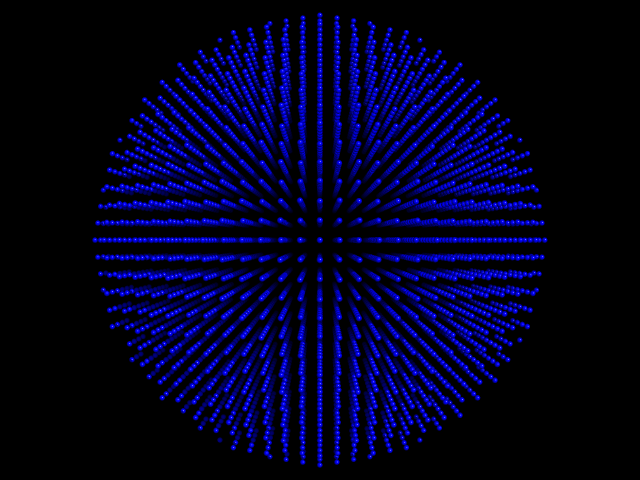
\includegraphics{figures/Xe5083rotation/png/Xe5083_0001.png}}{figures/Xe5083rotation/Xe5083rotation.swf}
		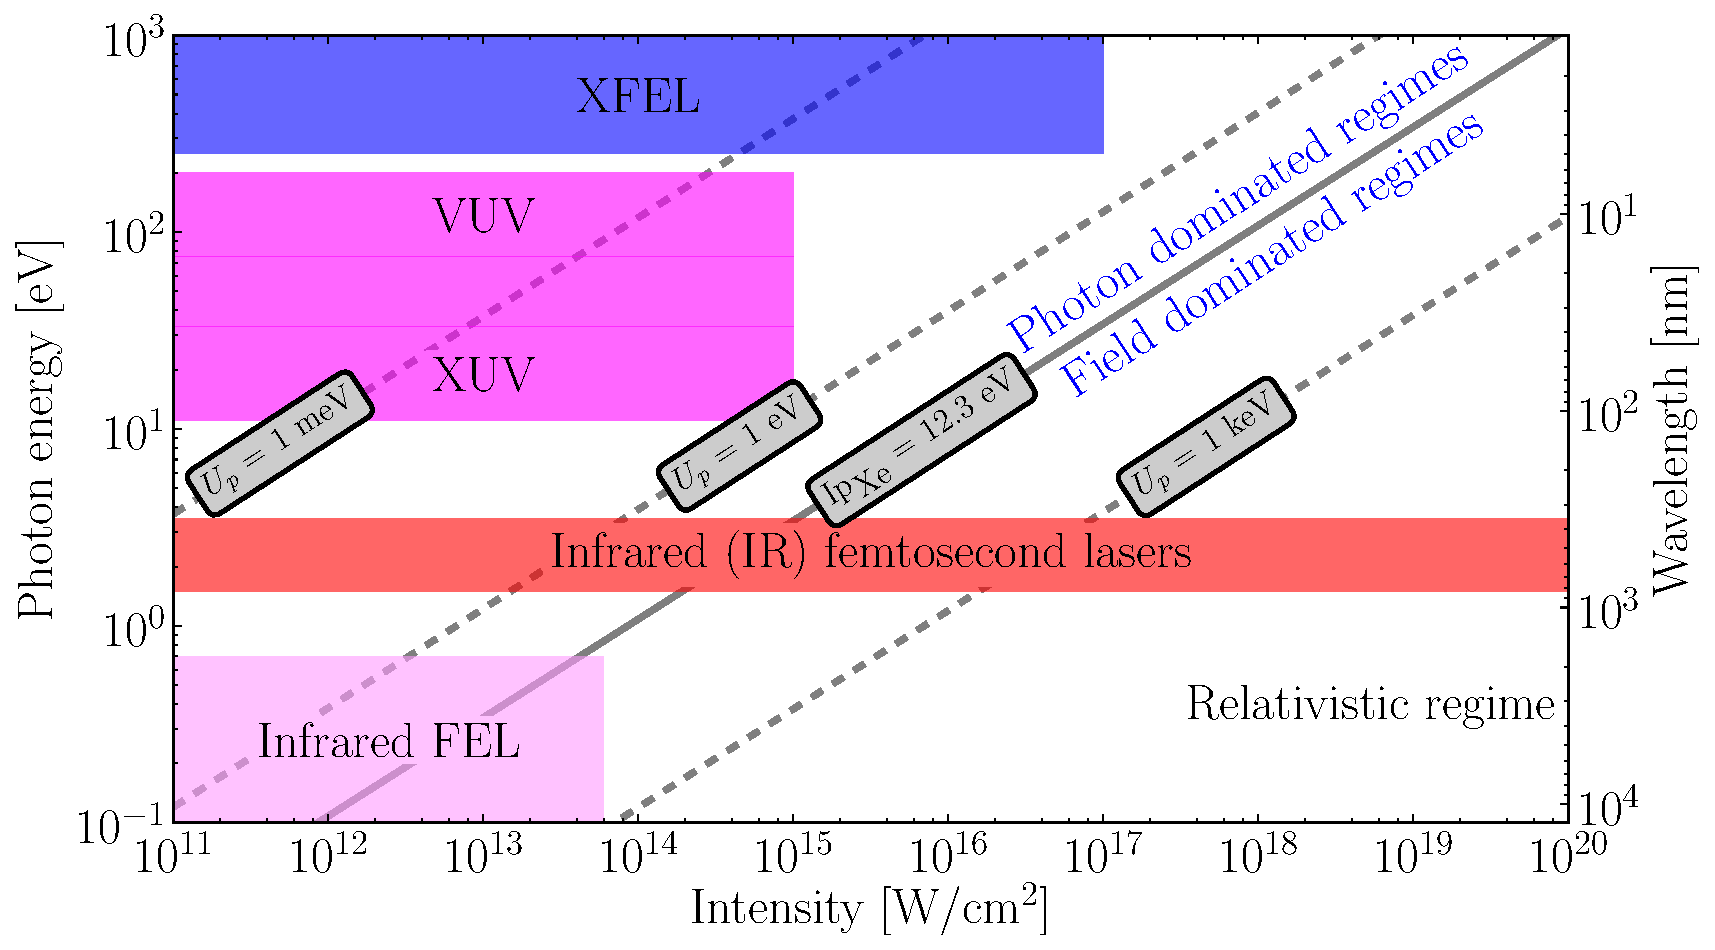
\includegraphics[width=1.1\textwidth]{../figures/regimes}
	\end{columns}
\end{frame}

% ***************************************************************
\subsection{Some experiments}
\begin{frame}{Short $\lambda$}\framenumber
	\begin{columns}
		\column{0.5\textwidth}
			\begin{itemize}
			\item Important experiments in 2002
			\item $\lambda$ = 98 nm, 12.65 eV (VUV), 100 fs, 2$\times$10$^{13}$~W/cm$^2$
			\item Xe$^{0\rightarrow1+}$ = 12.13 eV\\Where does higher CS come from?
			\end{itemize}
		\column{0.4\textwidth}
			\begin{figure}
			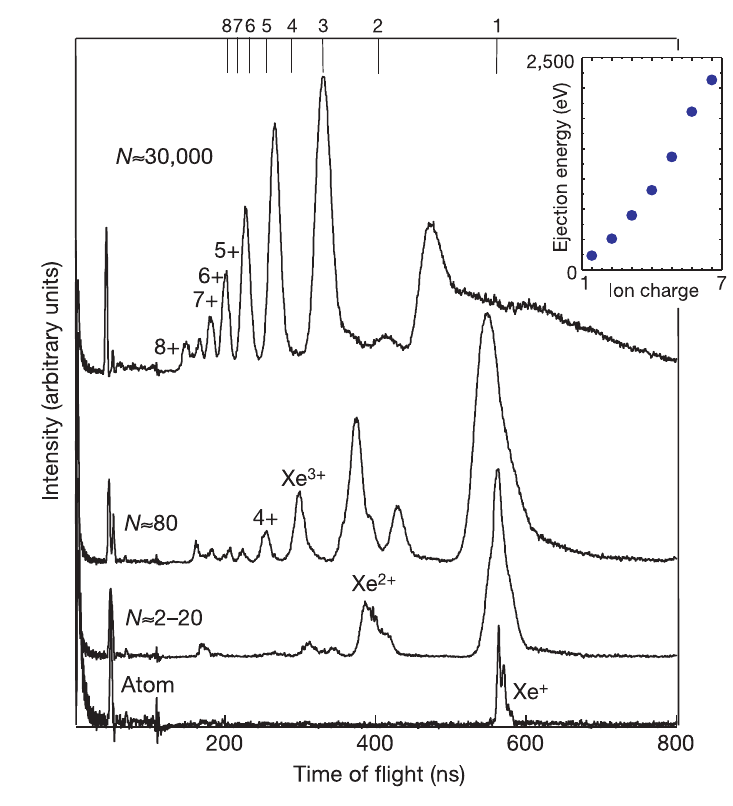
\includegraphics[width=\textwidth]{figures/Wabnitz2002_fig1}
			\caption{{\tiny Wabnitz \textit{et al}. Nature 420, 6915 482-5}}
			\end{figure}
	\end{columns}
\end{frame}




% ###############################################################
\section{Methodology}

% ---------------------------------------------------------------
\subsection{MD}
% ***************************************************************
\begin{frame}{}\framenumber
\begin{columns}
    \column{0.5\textwidth}
    Tool of choice: Molecular Dynamics (MD)
    \begin{itemize}
     \item Large field gradients
     \item Classical trajectories
     \item Simple algorithm
     \item Quantum effects
     \begin{itemize}
        \item Ionization (tunnel, photo-, impact)
        \item Excited states
     \end{itemize}
     \item<6-> MD code (>16k LoC)
     \item<6-> Ionization library (>18k LoC) and others
    \end{itemize}
    \column{0.5\textwidth}
    % Reserve space on frame 1
    \color{white}\only<1>{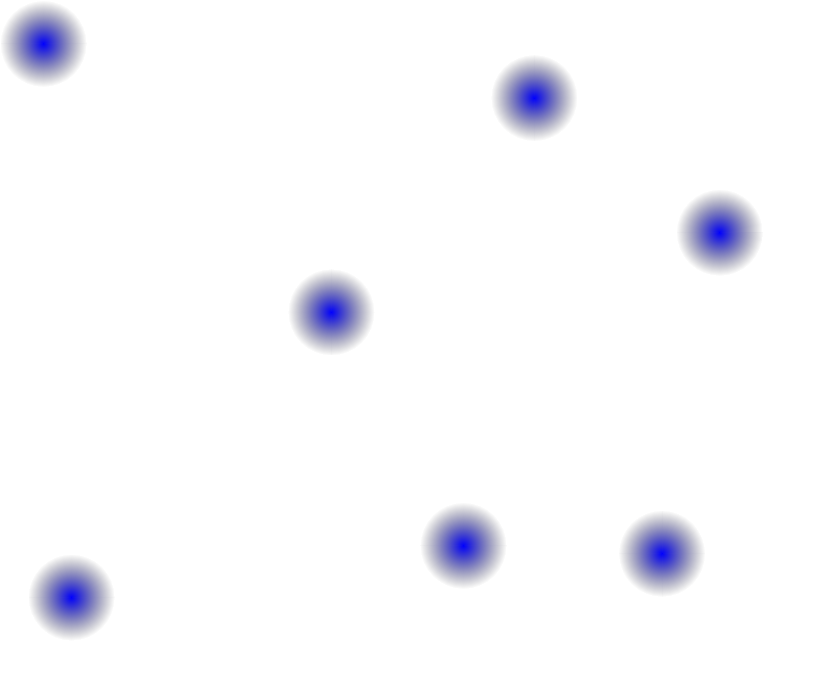
\includegraphics[draft,width=\textwidth]{figures/md_1}}\color{black}
    % http://tex.stackexchange.com/questions/55809/problem-with-only-and-alignment-of-graphics-pdf-in-beamer
    \only<2>{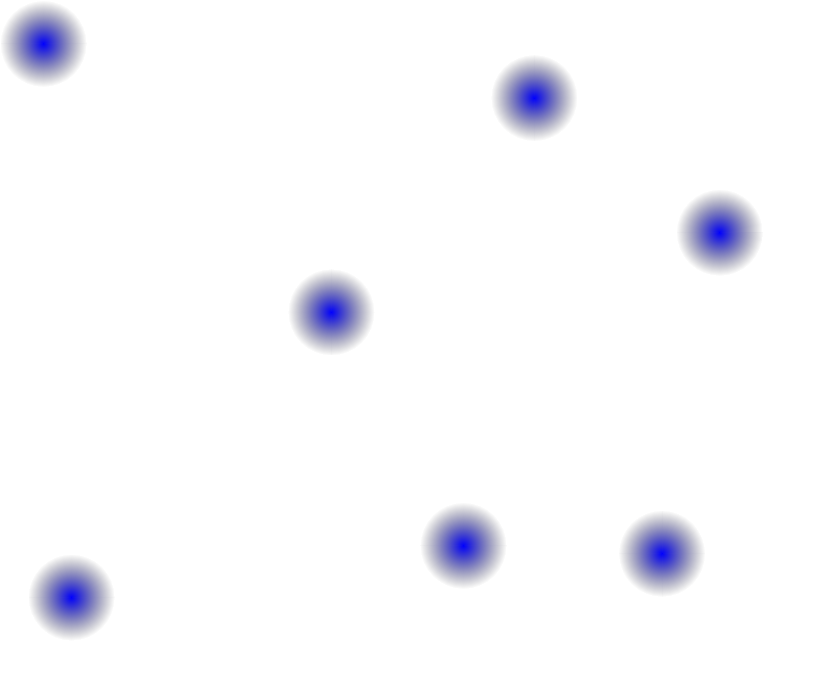
\includegraphics[width=\textwidth]{figures/md_1}}%
    \only<3>{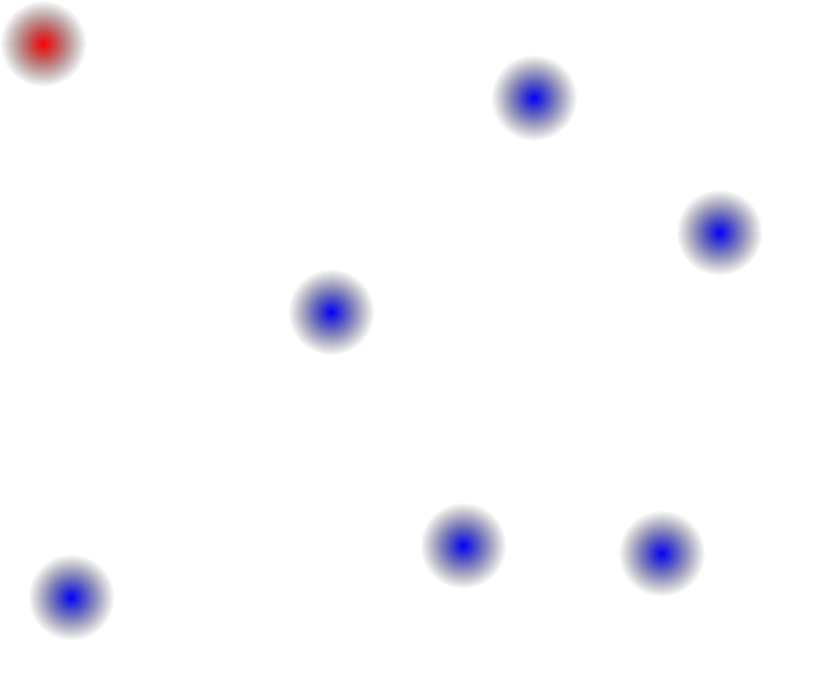
\includegraphics[width=\textwidth]{figures/md_2}}%
    \only<4>{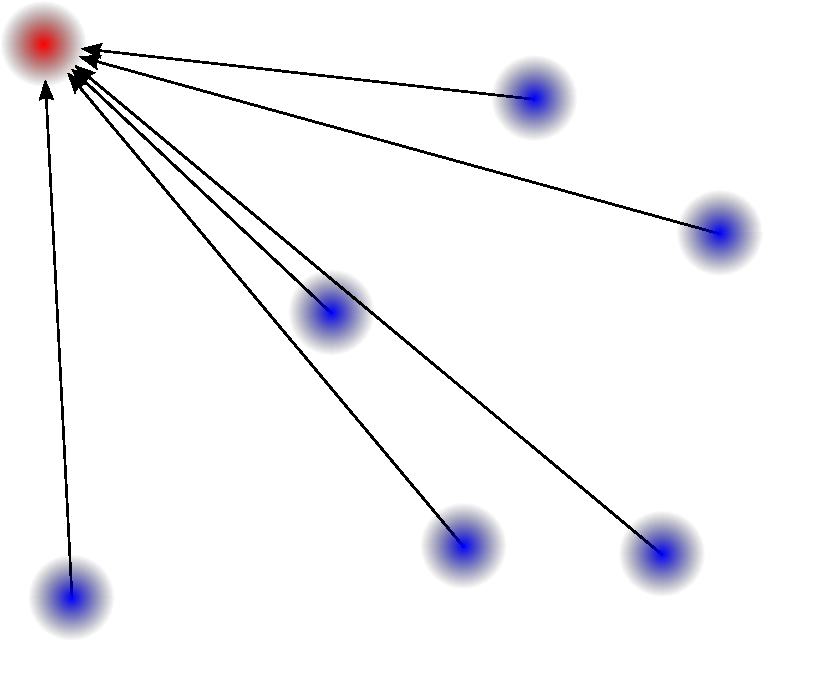
\includegraphics[width=\textwidth]{figures/md_3}}%
    \only<5->{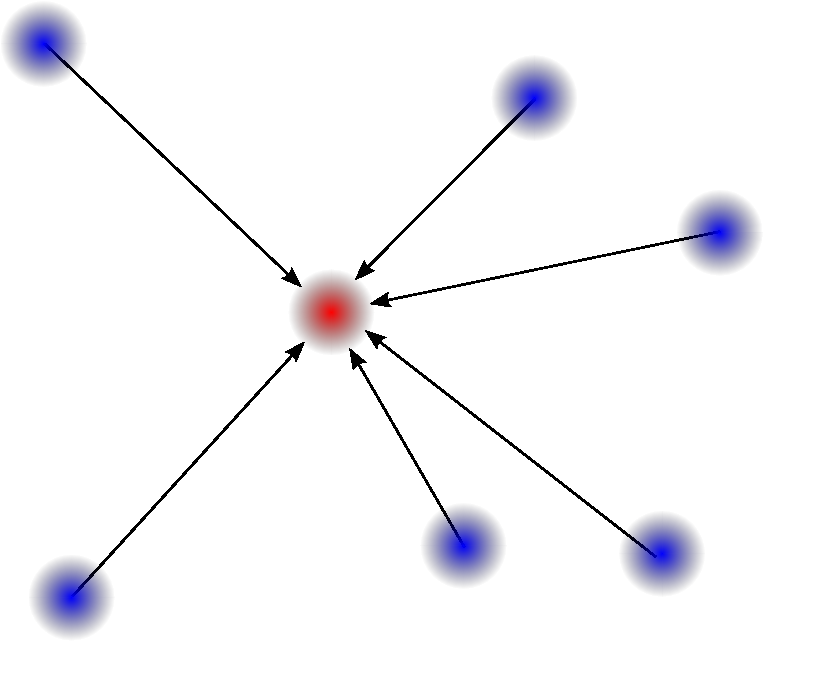
\includegraphics[width=\textwidth]{figures/md_4}}%
\end{columns}
\end{frame}

% ---------------------------------------------------------------
\subsection{Excited states}
% ***************************************************************
\begin{frame}{}\framenumber
\begin{columns}
    \column{0.5\textwidth}
        \begin{itemize}
        \item Suggested looking at excited states
        \item Previously ignored
        \item Developed a model:
            \begin{itemize}
            \item Two-step ionization process
            \item Rapid energy absorption + redistribution through clusters
            \end{itemize}
        \end{itemize}
    \column{0.55\textwidth}\centering
        %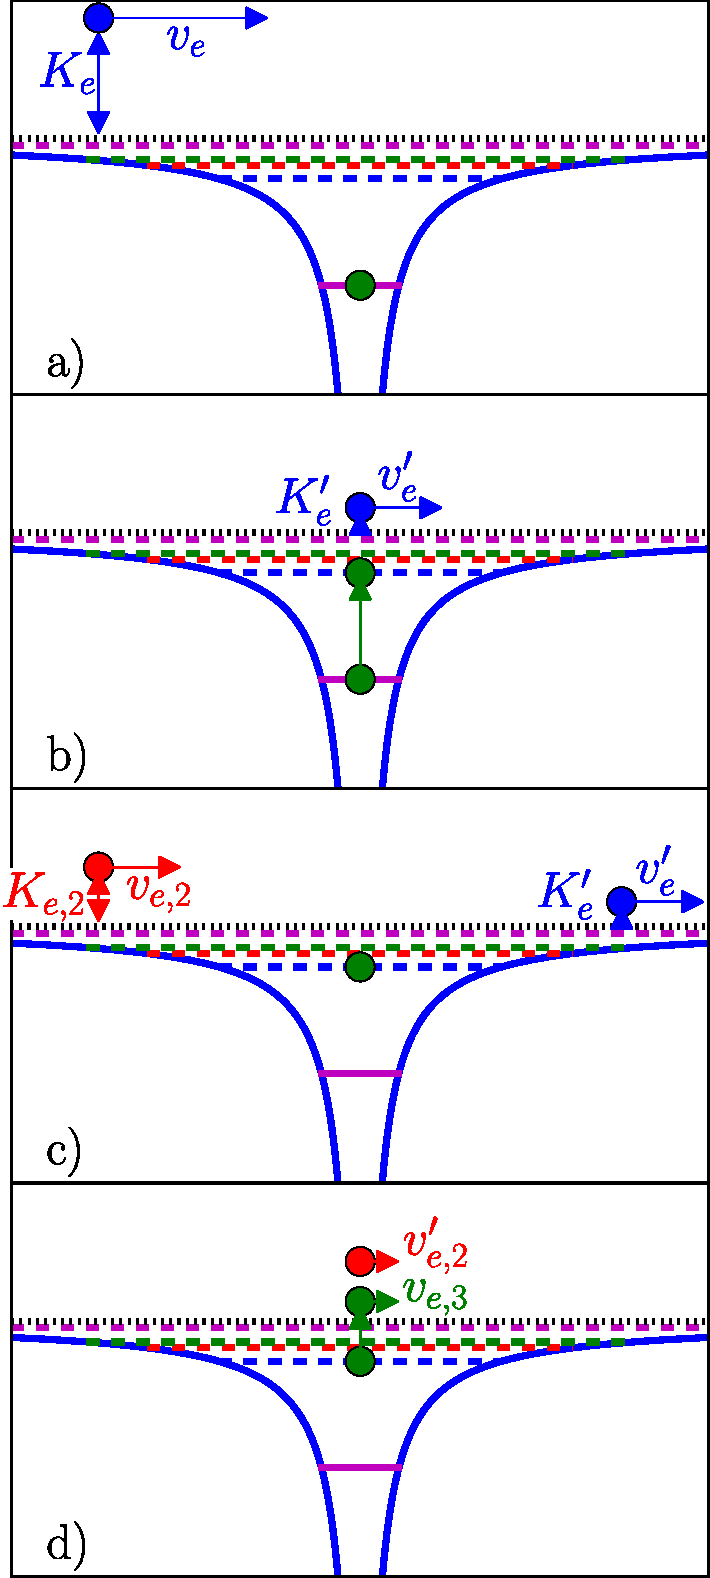
\includegraphics[width=0.6\textwidth]{figures/ionization_aci}
        \hspace{-21pt}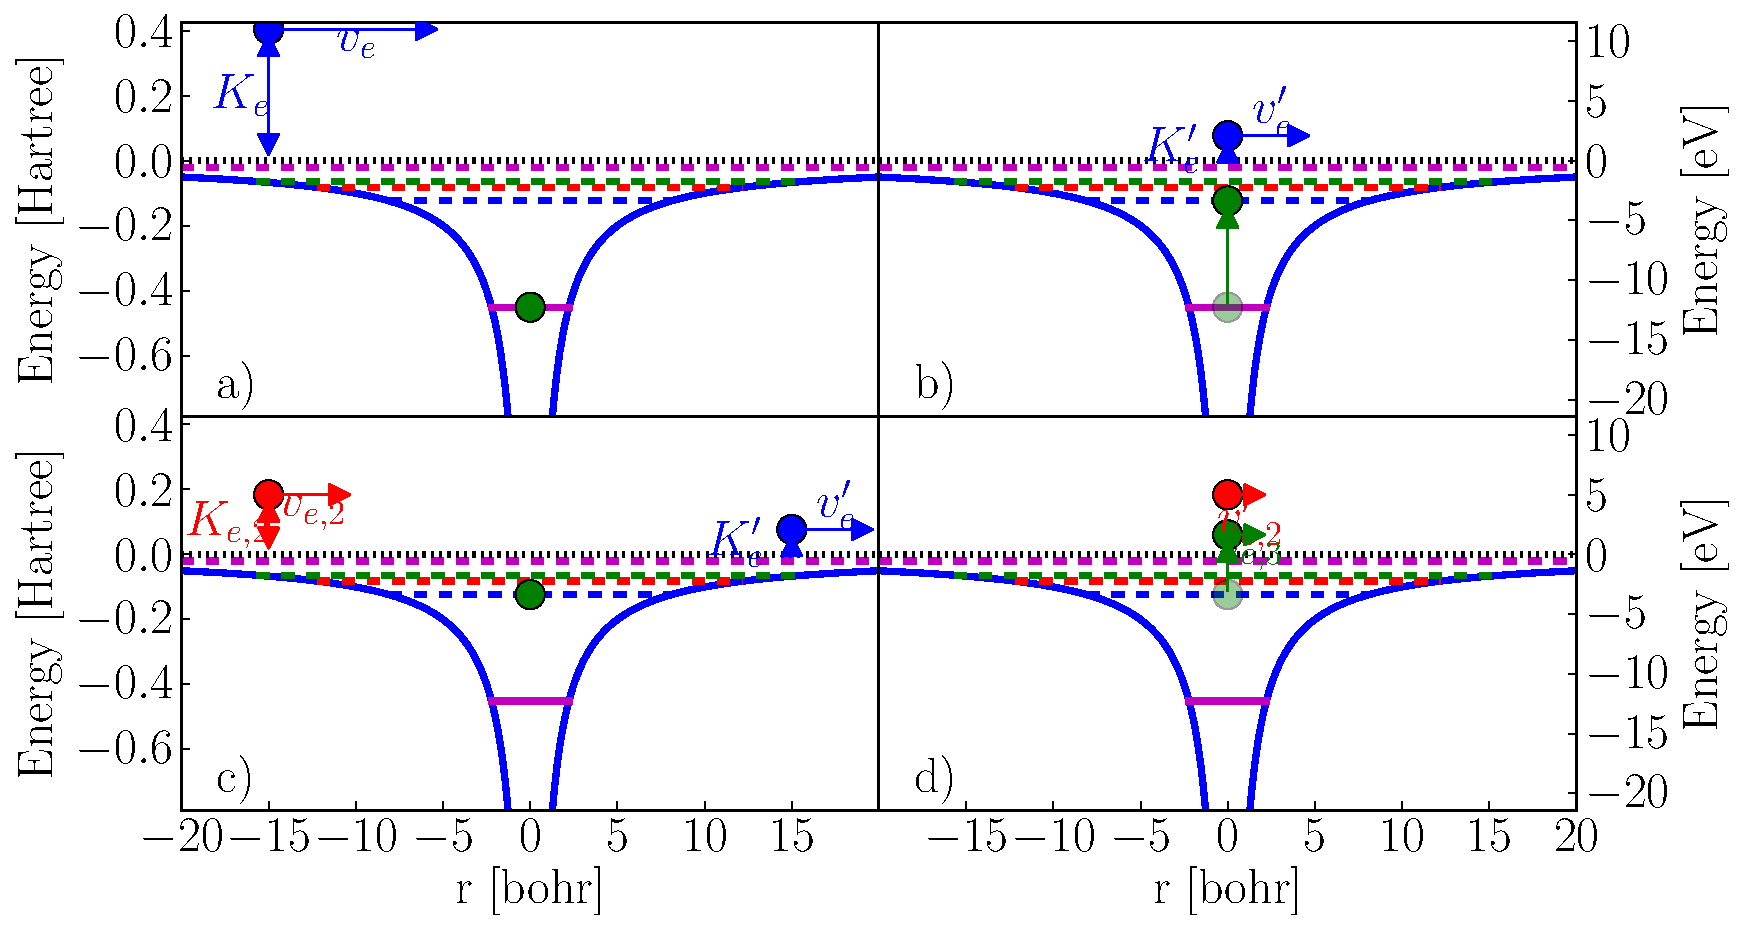
\includegraphics[width=1.1\textwidth]{../figures/ionization_aci} \\
        \hspace{-21pt}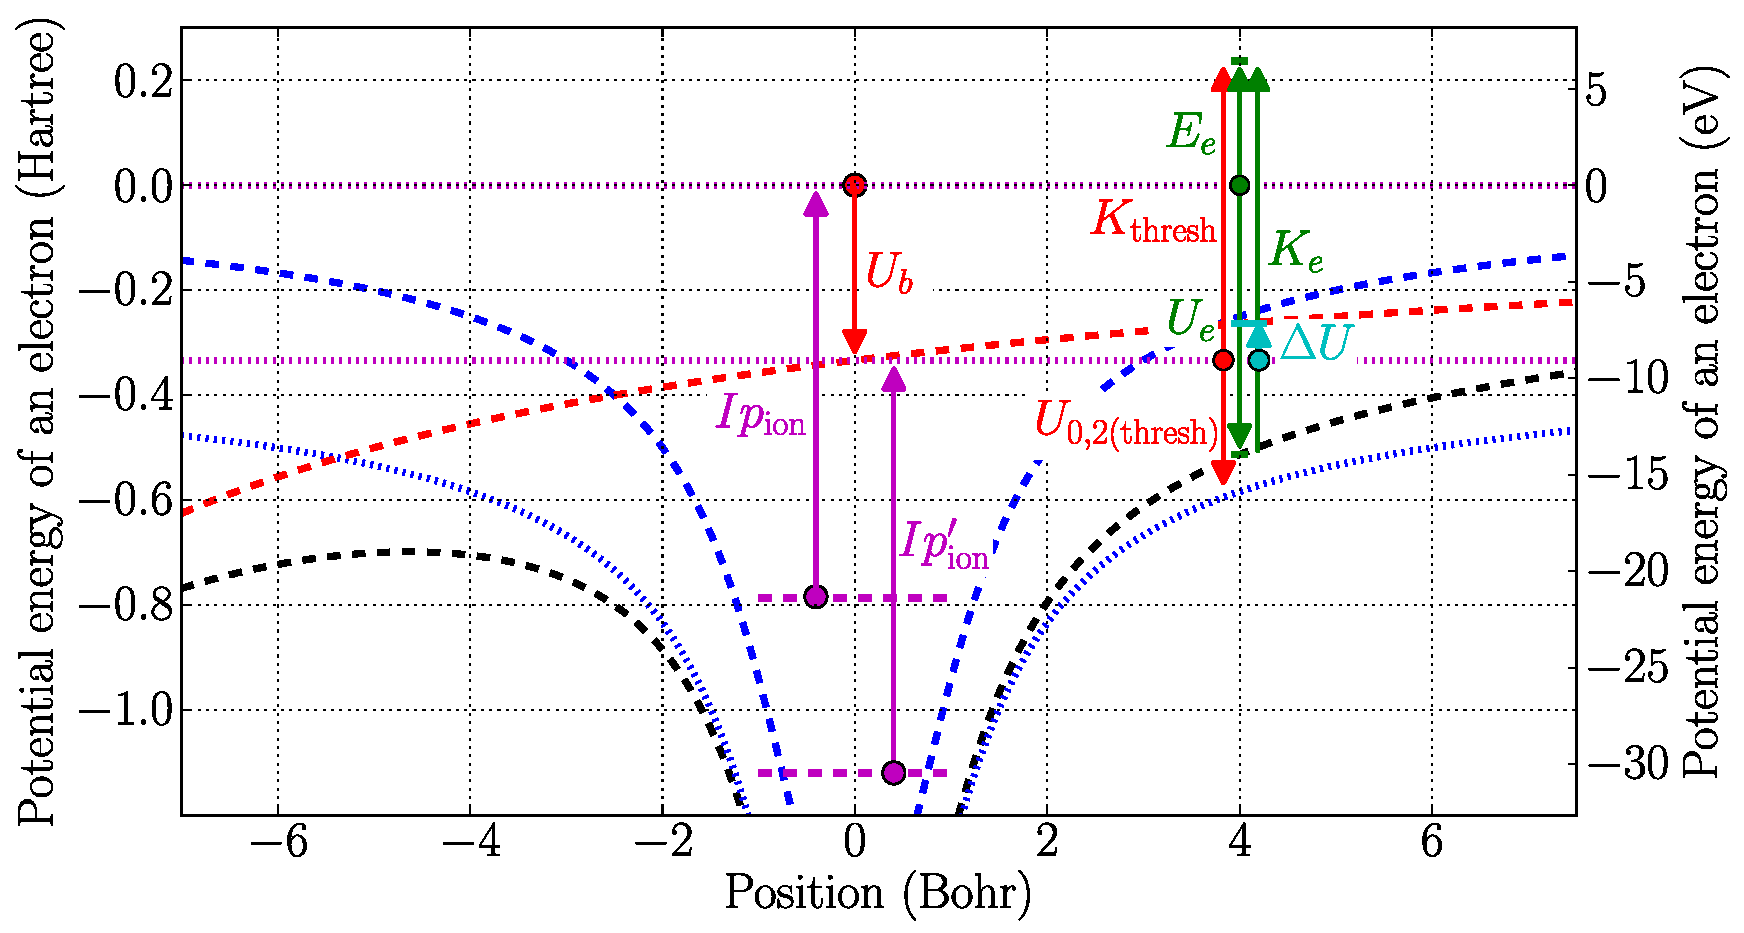
\includegraphics[width=1.1\textwidth]{figures/potential_landscape}
\end{columns}
{\uncover<2->{
\begin{textblock}{0.4}(0.5,0.52)\textblockcolour{white}\centering\textcolor{red}{
    \textbf{Augmented collisional ionization (ACI)}}
\end{textblock}
}}
\end{frame}

% ---------------------------------------------------------------
\subsection{Acceleration}
\begin{frame}{}\framenumber
\begin{columns}
    \column{0.5\textwidth}
    \begin{itemize}
     \item Hierarchical Tree algorithms
     \item General Purpose Graphical Processing Units (GP-GPU)
        \begin{itemize}
        \item CUDA vs OpenCL: Portability
        \item Refactoring
        \item Memory bandwidth and limit
        \item HPC Facilities
        \end{itemize}
    \end{itemize}

    \column{0.5\textwidth}
    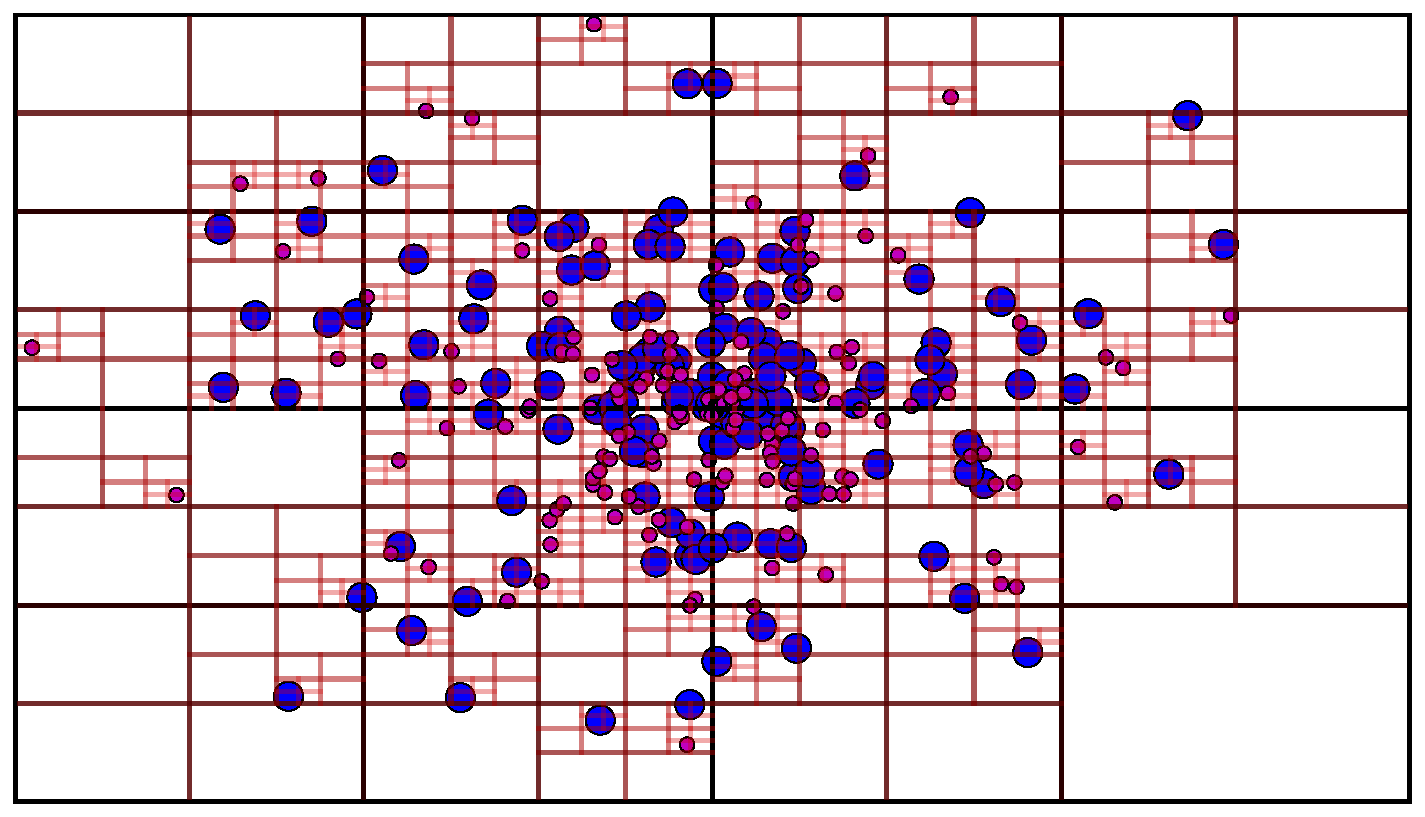
\includegraphics[width=\textwidth]{../figures/quadtree}\\
    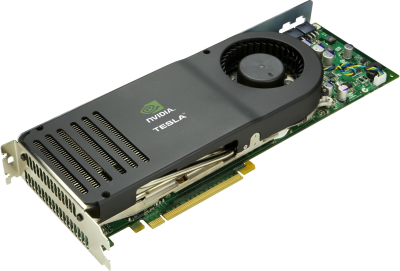
\includegraphics[width=\textwidth]{figures/tesla}


\end{columns}
\end{frame}

% ---------------------------------------------------------------
\subsection*{Example}
\begin{frame}{}\framenumber
% ffmpeg -i /home/nicolas/fichiers/documents/universite/doc/presentations.git/20120508_OCIP/movies/20110829_20h56_csec/mov%04d.png -qscale:v 1 -r 30 Xe1415_example.swf
\includemedia[label=H,activate=onclick,deactivate=onclick,width=\textwidth]
                {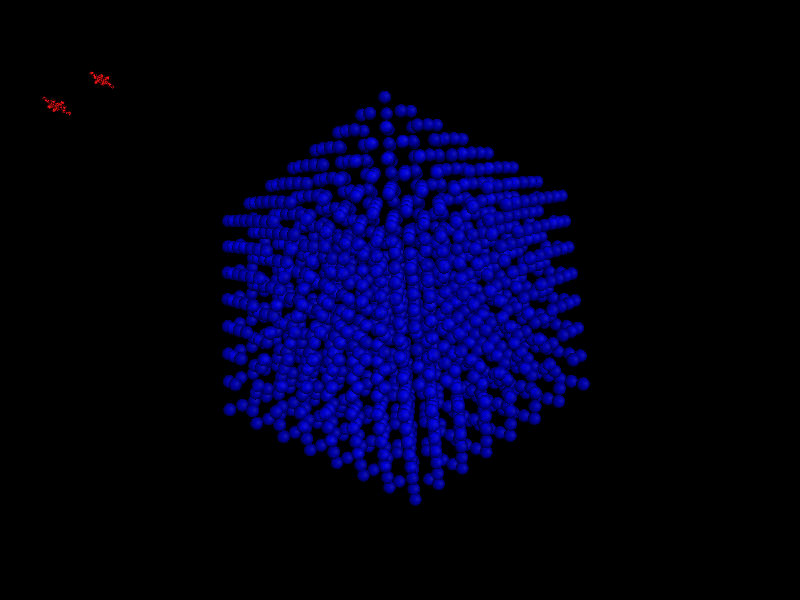
\includegraphics{figures/Xe_1415.png}}{figures/Xe1415_example.swf}
\end{frame}



% ###############################################################
\section{Studies}


% ---------------------------------------------------------------
\subsection{Argon @ XUV}
% ***************************************************************
\begin{frame}{}\framenumber
\begin{columns}
	\column{0.5\textwidth}
		\begin{itemize}
		\item 30~eV~regime~(30~nm)
			\begin{itemize}
			\item $E$ too small for inner shell ionization
			\item $E$ too large for field effects
			\end{itemize}
		\item Possible to isolate influence of internal electronic structures
		\begin{itemize}
			\item Single photon ionization starts dynamics
			\item Study the remaining...
		\end{itemize}
		\end{itemize}

	\column{0.5\textwidth}
		\begin{figure}
			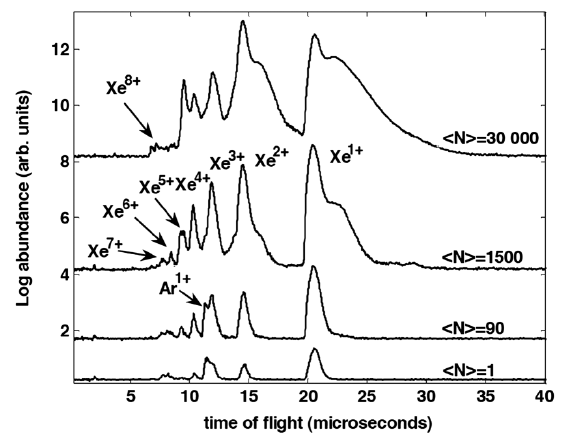
\includegraphics[width=\textwidth]{figures/Murphy2008_fig3}
			\caption{{\tiny Murphy \textit{et al.} PRL 101 (2008): 203401}}
		\end{figure}
\end{columns}
\end{frame}

% ***************************************************************
\begin{frame}{Results}\framenumber

%http://latex-beamer-class.10966.n7.nabble.com/Uncovering-figures-td1854.html
\setbeamercovered{invisible}

\begin{columns}
	\column{0.6\textwidth}
		\begin{itemize}
		\item Same parameters as Bostedt2008:
		\begin{itemize}
			\item 32.8 nm -- 38 eV
			\item $5\times10^{13} \rightarrow 5\times10^{14}$ W/cm$^2$
			\item 25 fs
			\item Ar$_{80}$, Ar$_{147}$
		\end{itemize}
		\item 1 ps duration (no significant changes after)
        \item<6-> {\color{red}$\rightarrow$ ACI most important process!}
		\end{itemize}

	\column{0.5\textwidth}
\begin{center}

\begin{textblock}{0.48}(0.515,0.27)
    \only<2>{     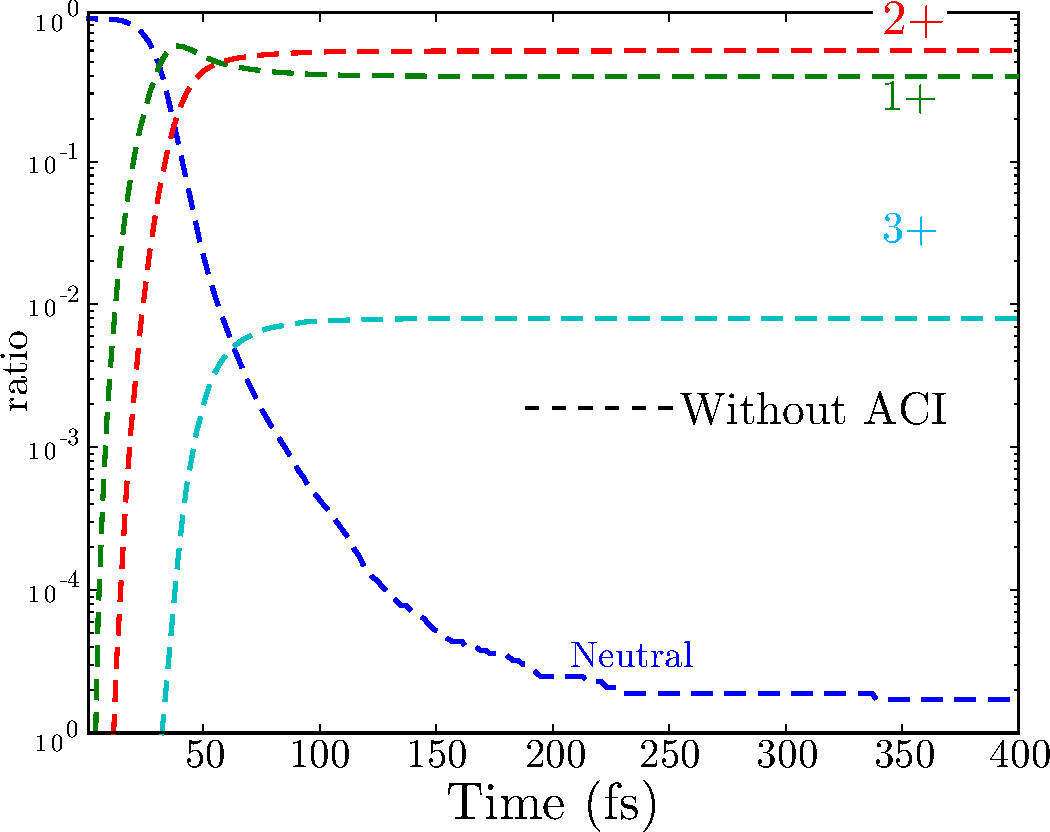
\includegraphics[width=\textwidth]{figures/cs_evolution_wo_aci} }
\end{textblock}
\begin{textblock}{0.48}(0.515,0.27)
    \only<3>{     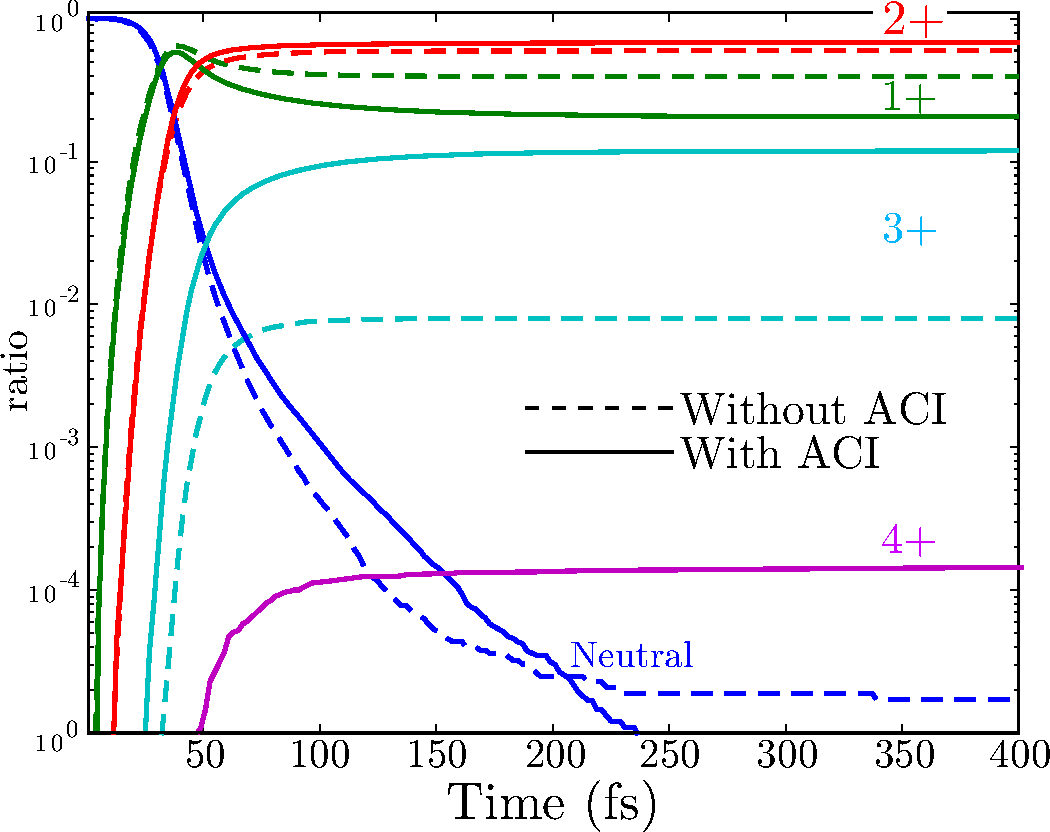
\includegraphics[width=\textwidth]{figures/cs_evolution_wo_and_w_aci} }
\end{textblock}
\begin{textblock}{0.48}(0.515,0.27)
    \only<4>{     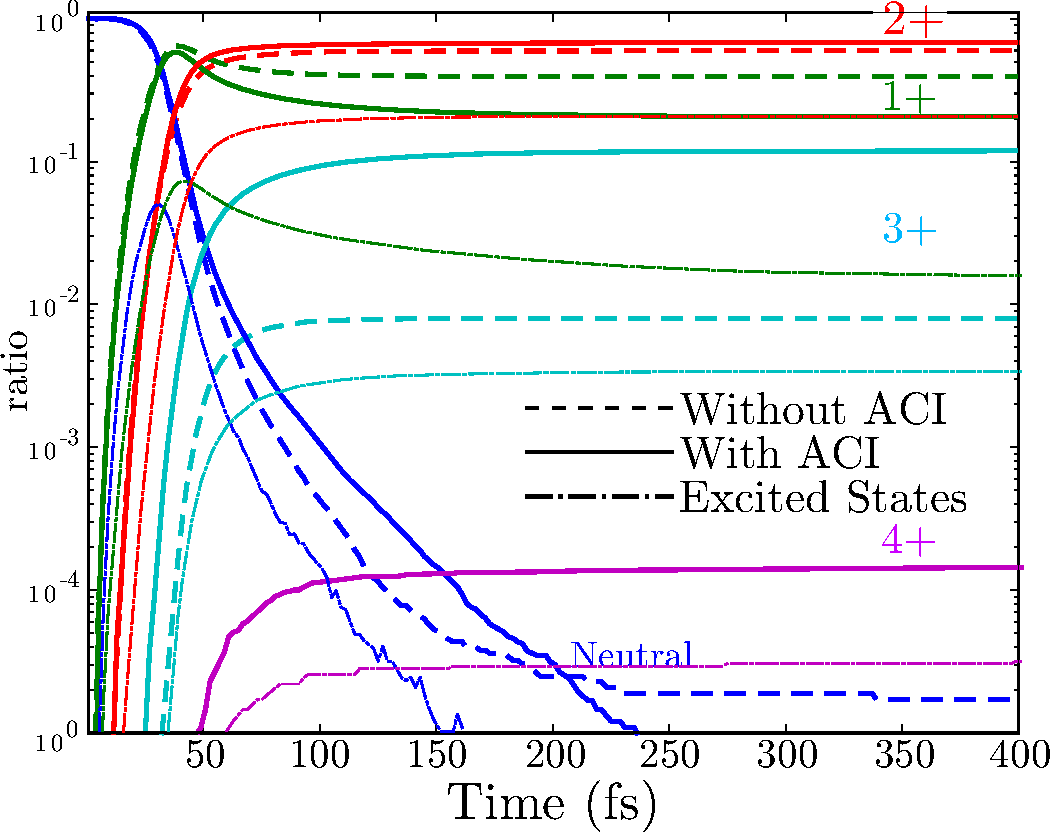
\includegraphics[width=\textwidth]{figures/cs_evolution_wo_and_w_aci_es} }
\end{textblock}
\begin{textblock}{0.2}(0.67,0.1)
    \only<5->{     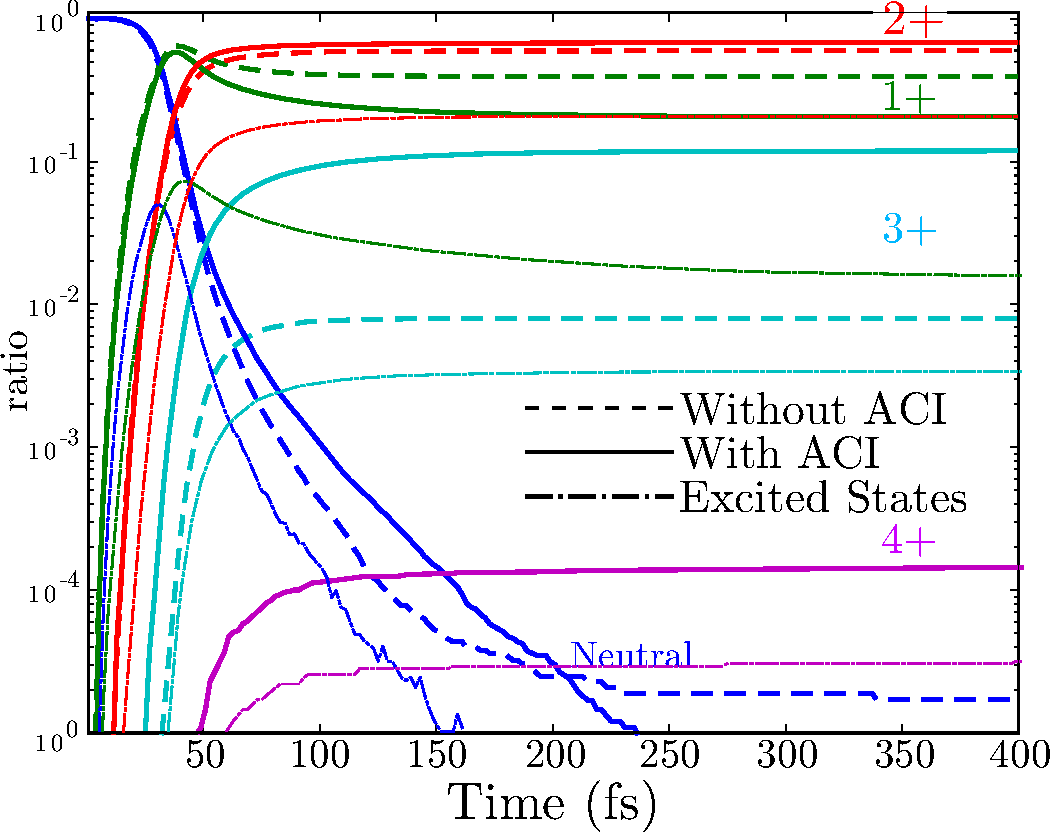
\includegraphics[width=\textwidth]{figures/cs_evolution_wo_and_w_aci_es} }
\end{textblock}
%
\begin{textblock}{0.48}(0.515,0.30)
    \only<5->{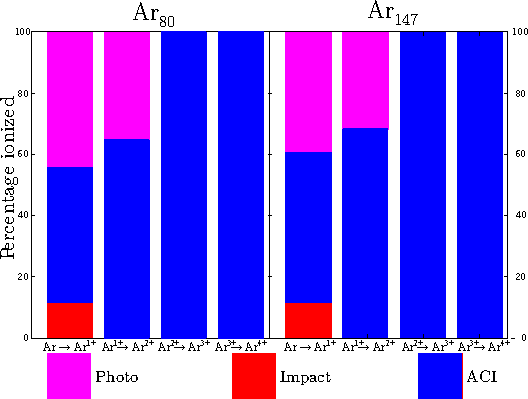
\includegraphics[width=\textwidth]{figures/ionization_relative}}
\end{textblock}

\end{center}

\end{columns}

\vspace{30pt}
{\begin{tiny}\uncover<7->{E. Ackad, N. Bigaouette, L. Ramunno. J. Phys. B, 44(16), 2011, 165102}\end{tiny}}
\end{frame}




% ###############################################################
\subsection{Cluster size}
\begin{frame}{}\framenumber\setbeamercovered{invisible}
    \begin{columns}
        \column{0.6\textwidth}
        \begin{itemize}
            \item<+-> Large clusters: $\searrow$ single-$\gamma$
            \item<+-> Q: Cluster size influence on explosion dynamics?
            \item<+-> Parameters:
            \begin{itemize}
                \item<.-> Ar$_{55}$, Ar$_{147}$, Ar$_{561}$ \& Ar$_{2057}$ (2, 3, 5, \& 8 shells)
                \item<.-> 32.8 nm -- 37.8 eV, 5$\times$10$^{13}$~W/cm$^2$, 25 fs
                \item<.-> 1 ps duration
                \item<+-> Single-$\gamma$: Only Ar$^{2+}$
            \end{itemize}
        \end{itemize}
        % Reserve space on frame 1
        %\only<1-4>{\color{white}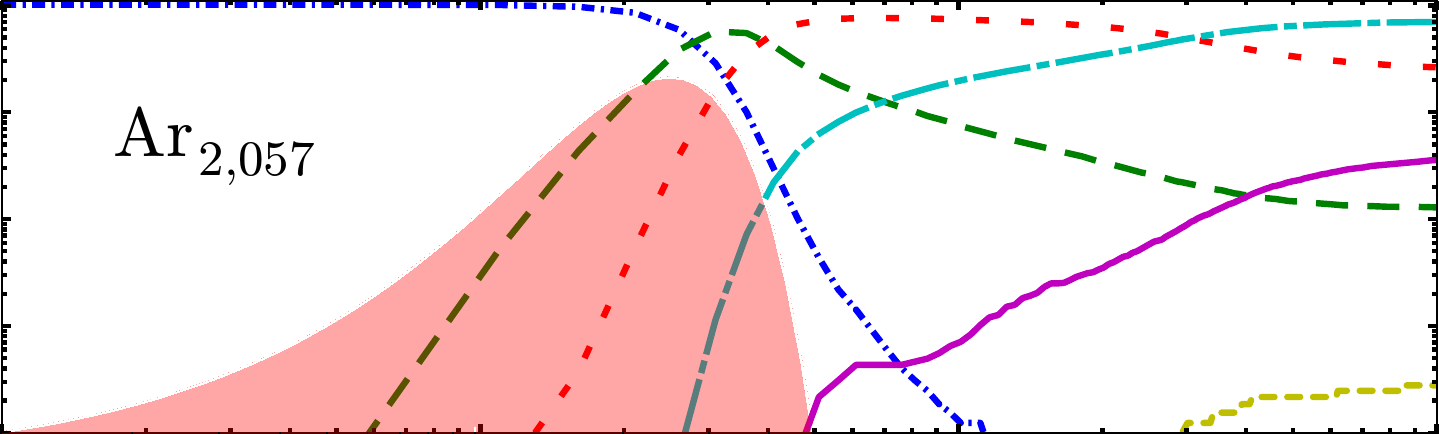
\includegraphics[width=\textwidth]{figures/Ackad2011b_fig3a}\color{black}}%
        \color{white}\only<1-4>{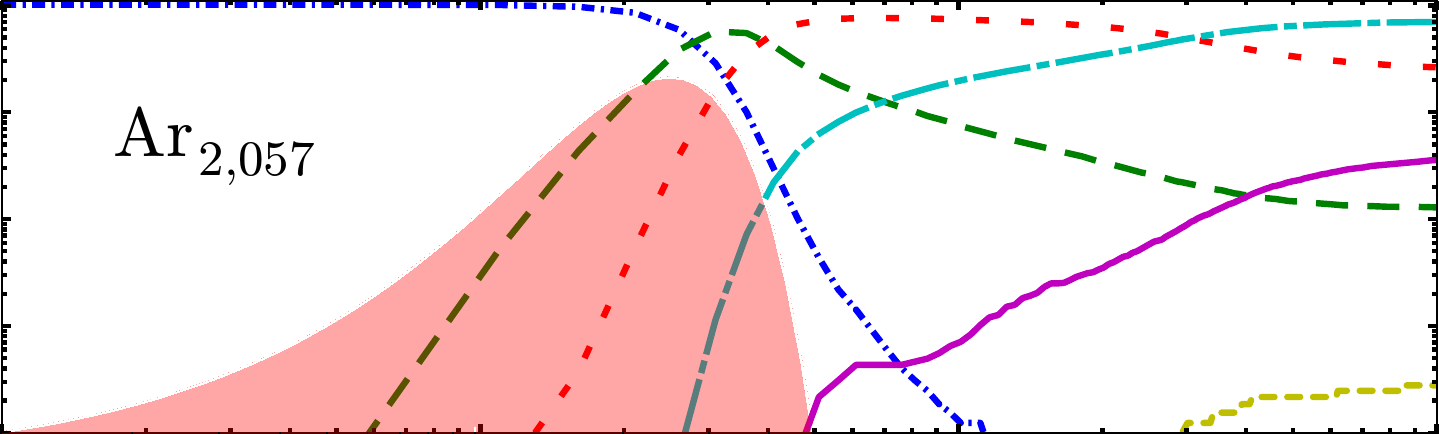
\includegraphics[draft,width=\textwidth]{figures/Ackad2011b_fig3a}}\color{black}
        \only<5>{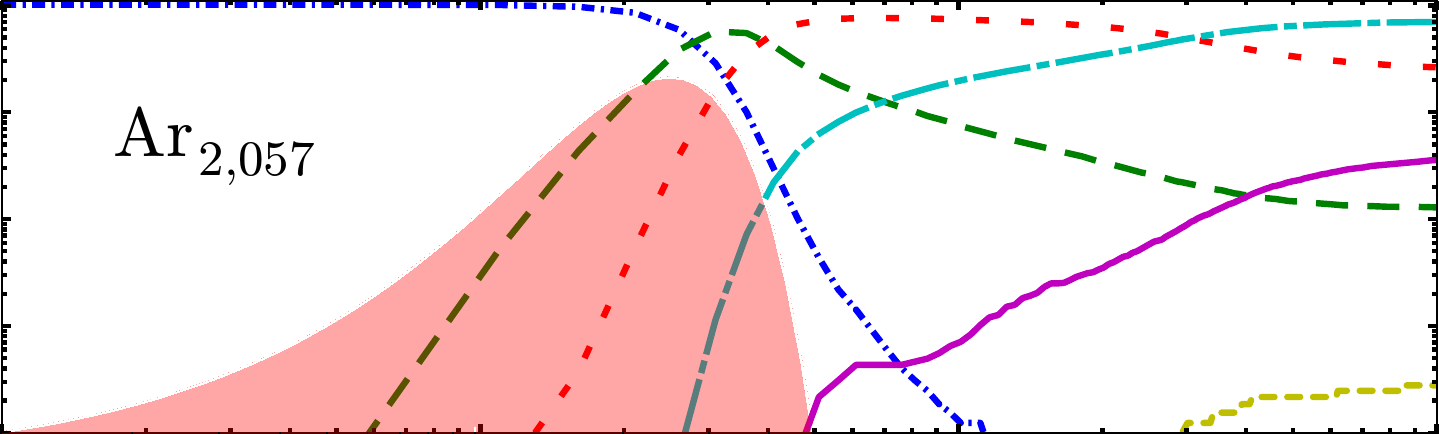
\includegraphics[width=\textwidth]{figures/Ackad2011b_fig3a}}%
        \only<6->{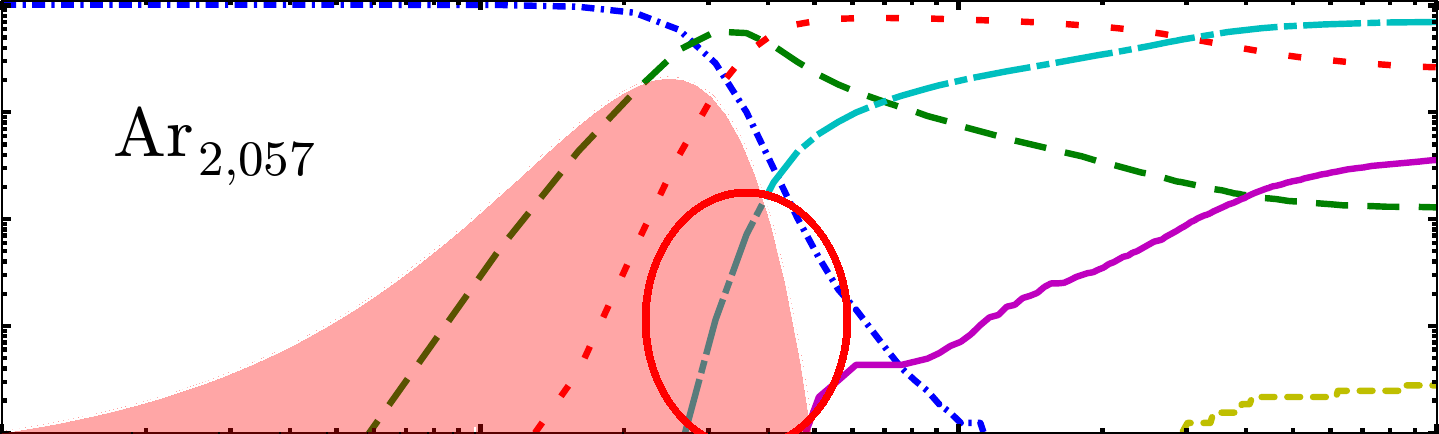
\includegraphics[width=\textwidth]{figures/Ackad2011b_fig3a_3plus}}

        \column{0.5\textwidth}
            \begin{itemize}
            \item<+-> <CS> $\nearrow$ with size:\\
            \uncover<.->{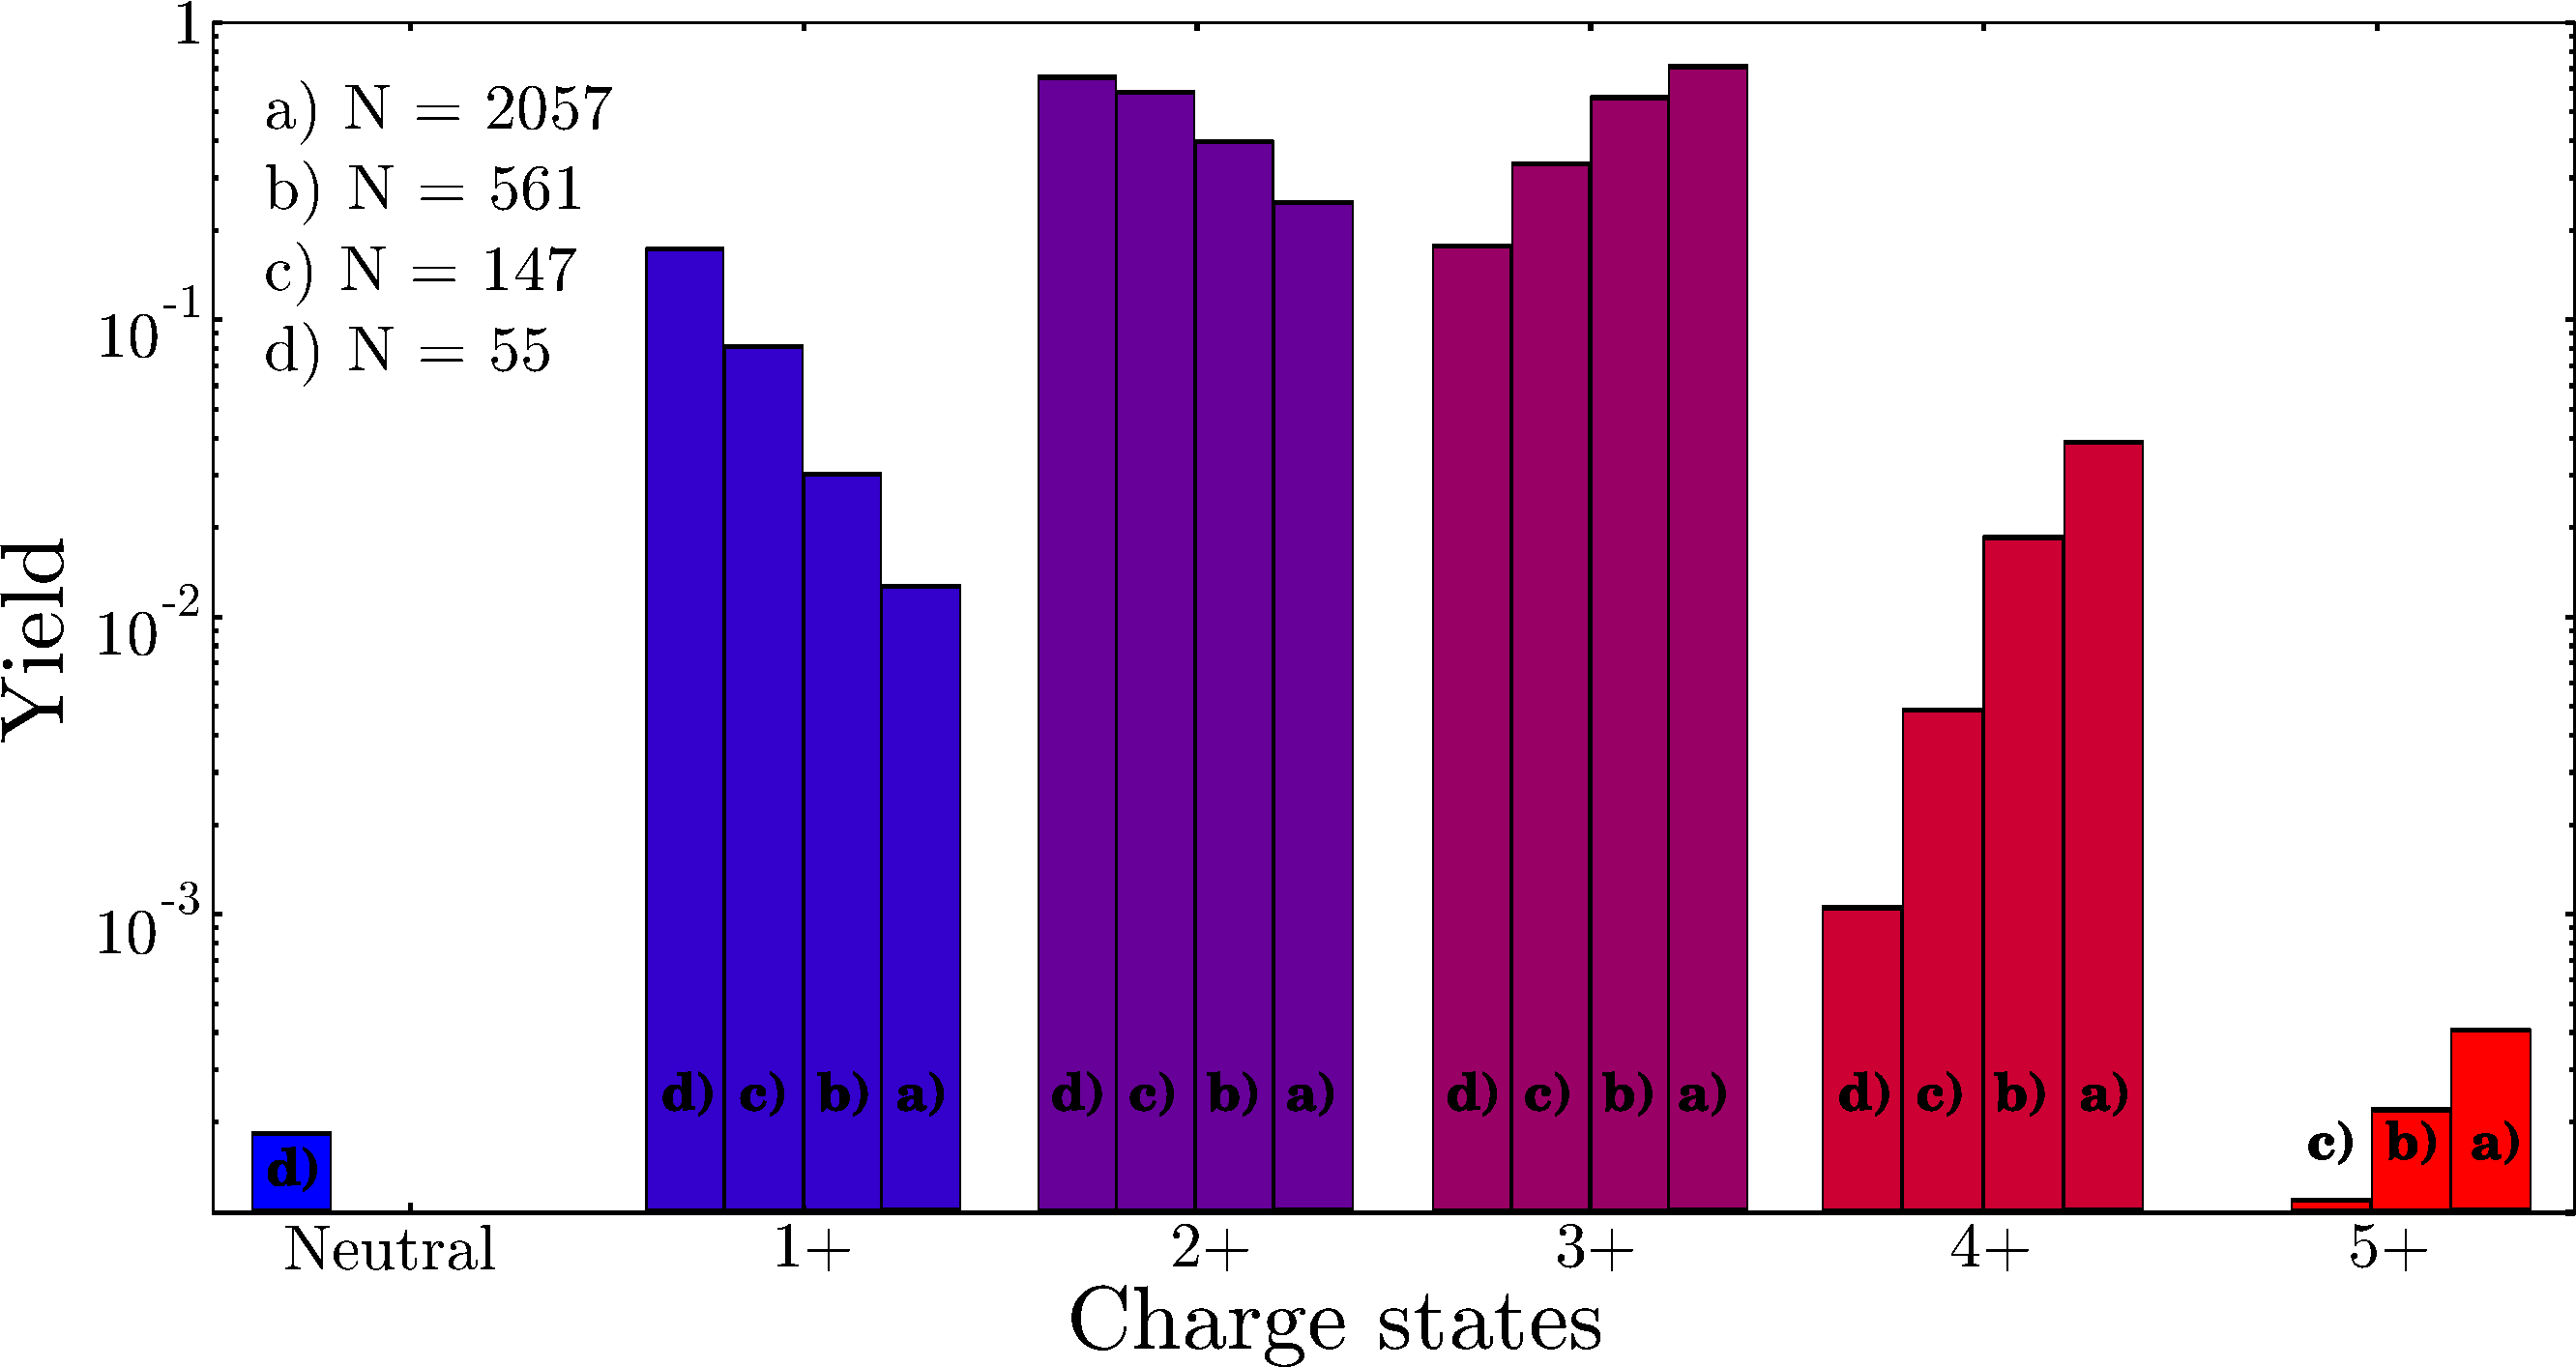
\includegraphics[width=0.9\textwidth]{figures/Ackad2011b_fig1}}\\%
            \item<.-> Even with $\searrow$ in $\gamma$/atom
            \item<+-> No IBH: High CS \textit{after} laser
            \item<.-> Ar$_{2,057}$: $\uparrow$CS $\Rightarrow$ $\emptyset~\gamma$
            \item<.-> $\searrow$ $\sim$40~\% $\gamma$
            \item<.-> Collisionally Reduced Photoabsorbtion (CRP)
            \end{itemize}
    \end{columns}

\uncover<+->{
    \begin{tiny}
    E. Ackad, N. Bigaouette, K. Briggs, L. Ramunno. Phys. Rev. A 83(6), 2011, 063201
    \end{tiny}
}
\end{frame}

% ###############################################################
\subsection{Xenon @ VUV}
% ---------------------------------------------------------------
\subsubsection{100 nm}
% ***************************************************************
\begin{frame}{}\framenumber
    \begin{columns}
        \column{0.6\textwidth}
        {\only<1>{   Wabnitz2002 (2$\times$10$^{13}$~W/cm$^2$):\\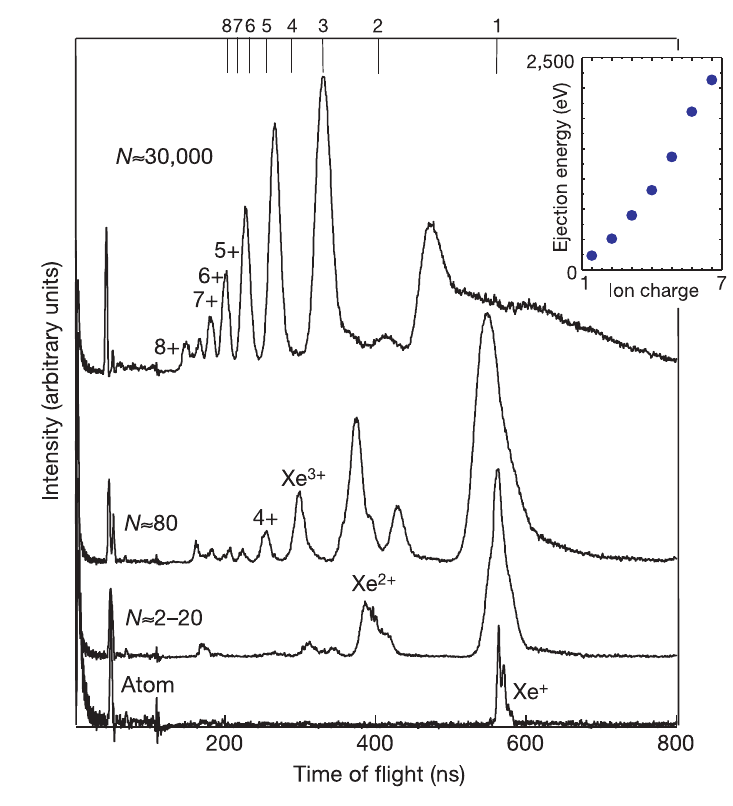
\includegraphics[width=\textwidth]{figures/Wabnitz2002_fig1}}}%
        {\only<2-3>{ Bostedt2010 (8$\times$10$^{12}$~W/cm$^2$):\\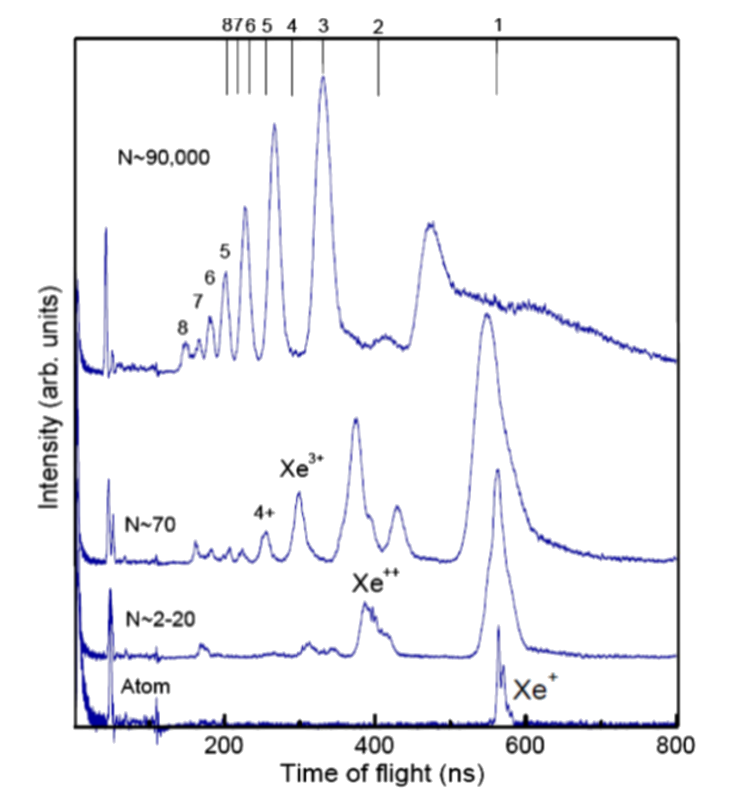
\includegraphics[width=\textwidth]{figures/Bostedt2010_fig2}}}%
        {\only<4->{  Bostedt2010 (8$\times$10$^{12}$~W/cm$^2$):\\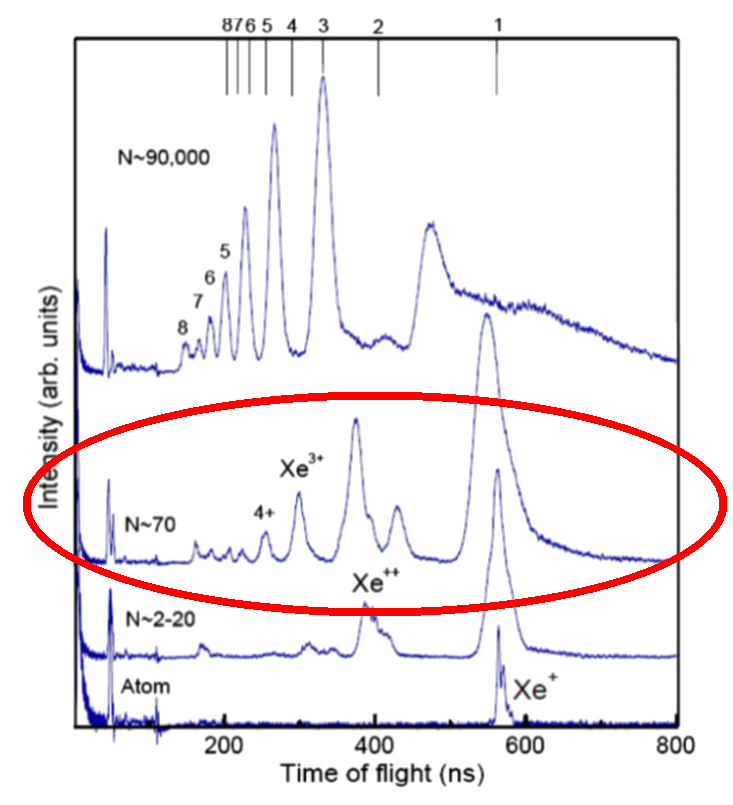
\includegraphics[width=\textwidth]{figures/Bostedt2010_fig2_Xe70}}}%

        \column{0.5\textwidth}
        \begin{itemize}
            \item<1-> 98 nm -- 12.65 eV, 100~fs
            \item<2-> Reduced ($\sim$40\%) intensity
            \item<3-> Can ACI explain high CS seen?
        \end{itemize}

    \end{columns}
\end{frame}

% ***************************************************************
\begin{frame}{I = 8$\times$10$^{12}$ W/cm$^2$}\framenumber
\setbeamercovered{invisible}
%charge_states_statistic_Xe100nmPart2BodstedIntensityScan_N00090_I08e12_linear
\begin{columns}
    \column{0.5\textwidth}
    \begin{center}{\uncover<1->{Without ACI:\newline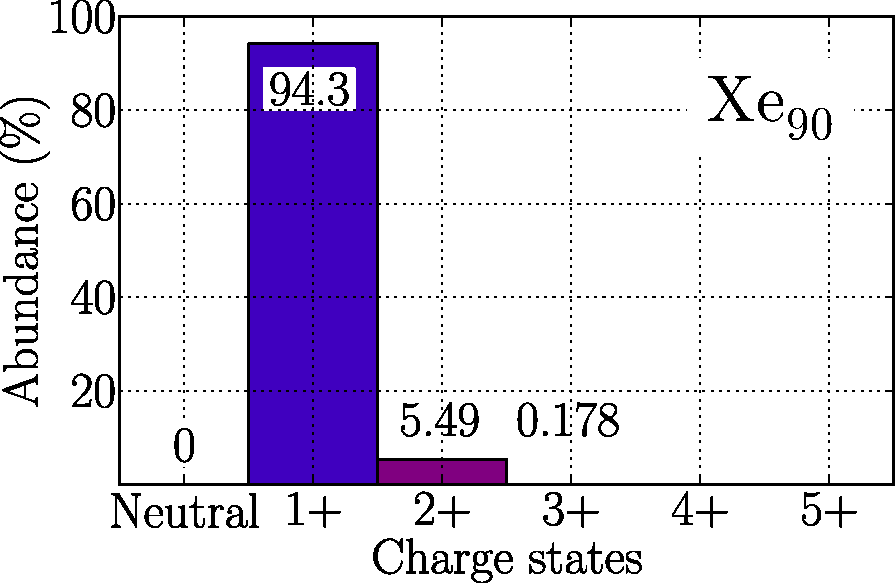
\includegraphics[width=\textwidth]{figures/cs_Xe100nm_N90_I8e12_wo_ACI}}}\end{center}
    \column{0.5\textwidth}
    \begin{center}{\uncover<2->{With ACI:\newline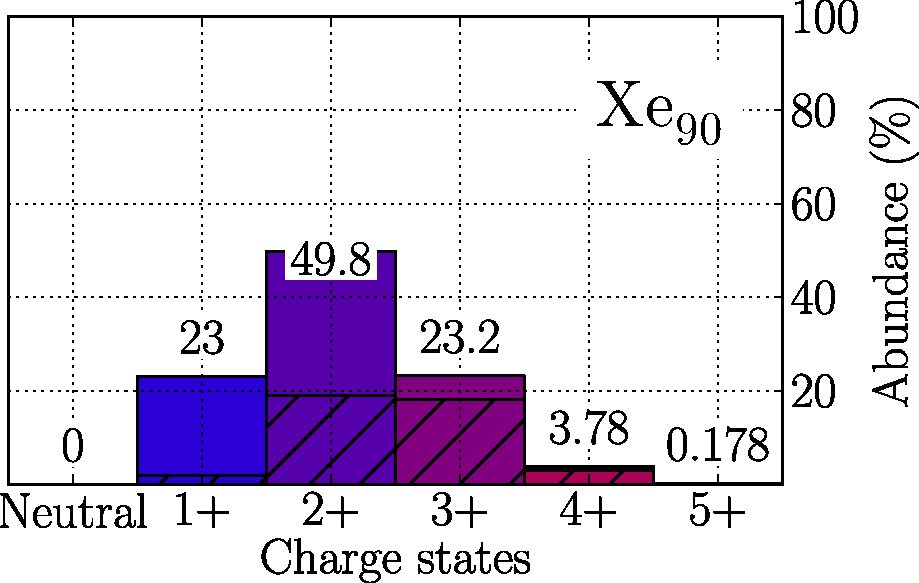
\includegraphics[width=\textwidth]{figures/cs_Xe100nm_N90_I8e12_w_ACI}}}\end{center}
\end{columns}
\begin{itemize}
    \item<2-> Max CS: Increased from Xe$^{2+}$ $\rightarrow$ Xe$^{4+}$
    \item<2-> Wabnitz2002: Siginificant signal for Xe$^{4+}$
    \item<2-> Large proportion in excited state
\end{itemize}
\end{frame}

% % ***************************************************************
% \begin{frame}{I = 5.6$\times$10$^{12}$ W/cm$^2$ (1.4$\times$10$^{13}$ @ 40\%)}\framenumber
%     \setbeamercovered{invisible}
%     % Primus:
%     % ./post_processing/charge_states_statistics.py --both --final --linear --params=Eno --params=Eyes --conf=0.07,0.07,0.17,0.02,0.0,0.1 --output=/raid/nicolas/md/20131016_19h31_100nmExtraDefense --save -i 20131110_21h06*Xe100nmExtraRunsDefense*nbions01415*I05.6000e+12
%     \begin{columns}
%         \column{0.5\textwidth}
%         \begin{center}{\uncover<1->{Without ACI:\newline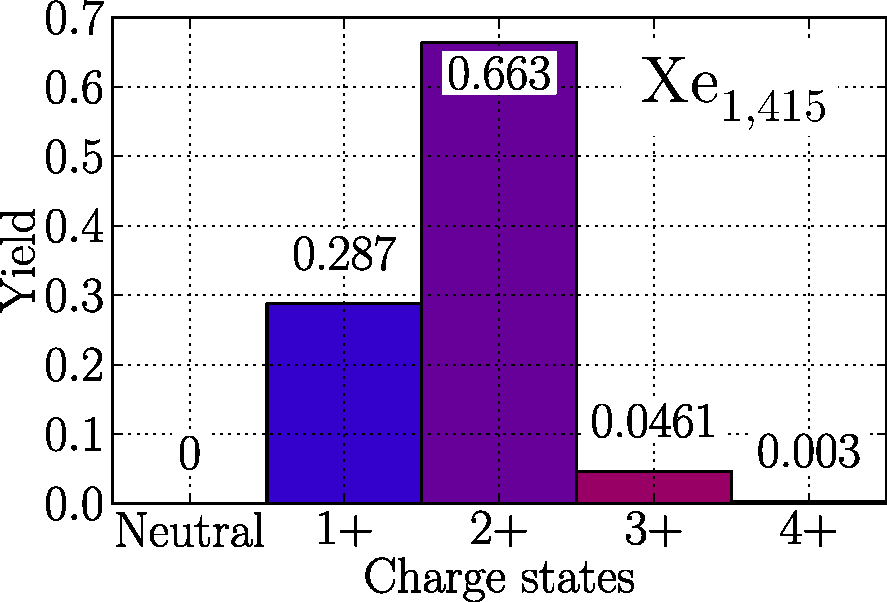
\includegraphics[width=\textwidth]{figures/charge_states_statistic_20131110_21h06Xe100nmExtraRunsDefensenbions01415_I56e11_linear_ACI_OFF}}}\end{center}
%         \column{0.5\textwidth}
%         \begin{center}{\uncover<2->{With ACI:\newline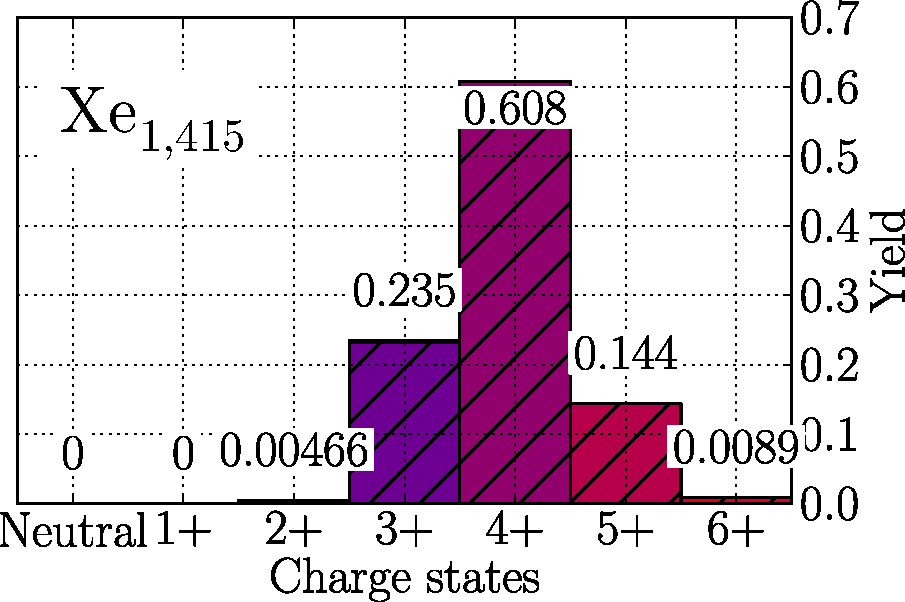
\includegraphics[width=\textwidth]{figures/charge_states_statistic_20131110_21h06Xe100nmExtraRunsDefensenbions01415_I56e11_linear_ACI_ON}}}\end{center}
%     \end{columns}
%     \begin{center}{
%     \uncover<3->{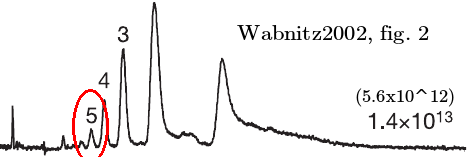
\includegraphics[width=0.5\textwidth]{figures/Wabnitz2002_fig2_1p4e13_Xe5p}}}
%     \end{center}
% \end{frame}
\begin{frame}{I = 1.5$\times$10$^{13}$ W/cm$^2$}\framenumber
    \setbeamercovered{invisible}
    % charge_states_statistic_Xe100nmPart1ComparisonCJ_N01000_I1512_linear
    \begin{columns}
        \column{0.5\textwidth}
        \begin{center}{\uncover<1->{Without ACI:\newline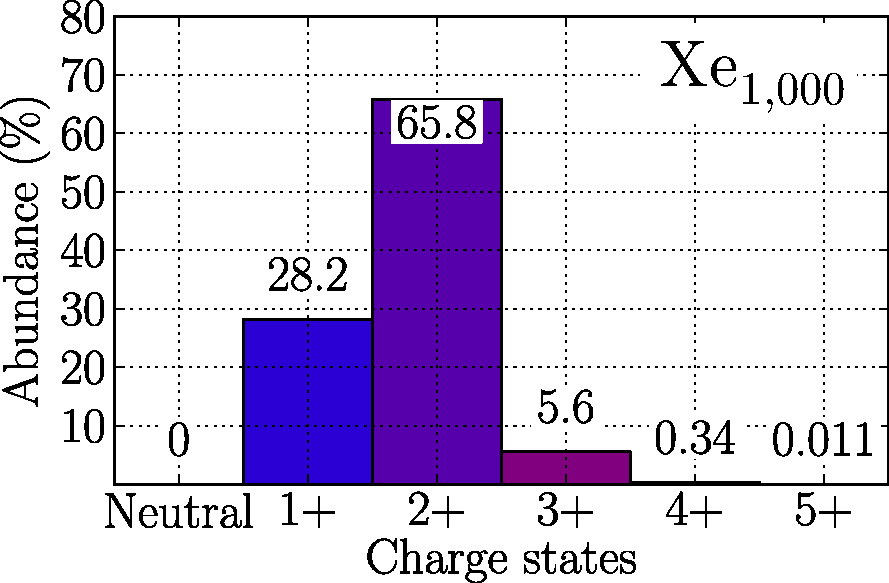
\includegraphics[width=\textwidth]{figures/charge_states_statistic_Xe100nmPart1ComparisonCJ_N01000_I1512_linear_ACI_OFF}}}\end{center}
        \column{0.5\textwidth}
        \begin{center}{\uncover<2->{With ACI:\newline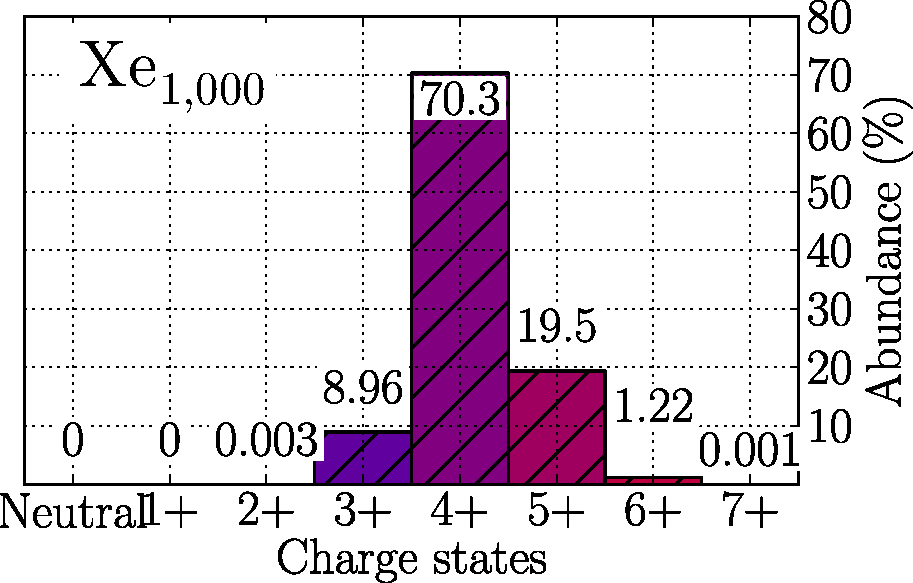
\includegraphics[width=\textwidth]{figures/charge_states_statistic_Xe100nmPart1ComparisonCJ_N01000_I1512_linear_ACI_ON}}}\end{center}
    \end{columns}
    \begin{center}{
    \uncover<3->{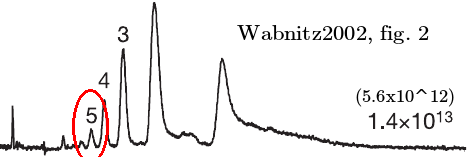
\includegraphics[width=0.5\textwidth]{figures/Wabnitz2002_fig2_1p4e13_Xe5p}}}
    \end{center}
\end{frame}


% 1415 is too small
% % ***************************************************************
% \begin{frame}{Spatial averaging (@ 8$\times$10$^{12}$ W/cm$^2$)}\framenumber
%     \setbeamercovered{invisible}
%     \begin{columns}
%         \column{0.5\textwidth}
%         \begin{center}{\uncover<1->{Without ACI:\newline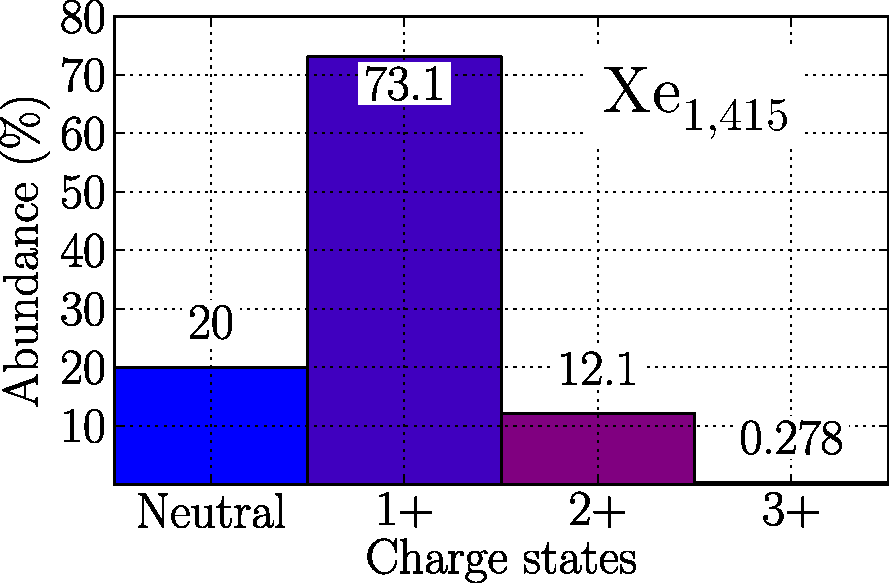
\includegraphics[width=\textwidth]{figures/figure_results_part2_CS_Xe100nmPart2BodstedIntensityScan_N01415_linear_ACI_OFF}}}\end{center}
%         \column{0.5\textwidth}
%         \begin{center}{\uncover<2->{With ACI:\newline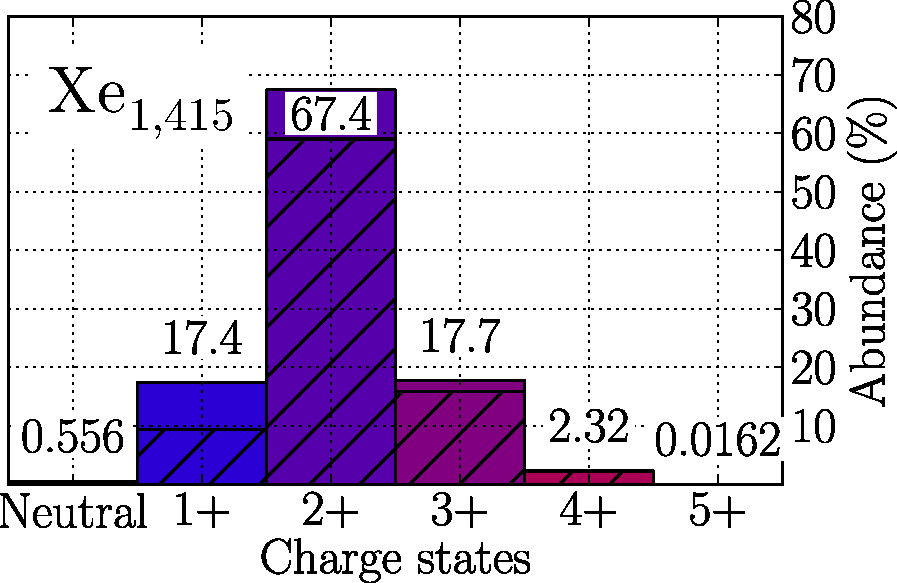
\includegraphics[width=\textwidth]{figures/figure_results_part2_CS_Xe100nmPart2BodstedIntensityScan_N01415_linear_ACI_ON}}}\end{center}
%     \end{columns}
%     \begin{center}{
%     \uncover<3->{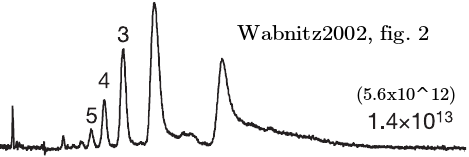
\includegraphics[width=0.5\textwidth]{figures/Wabnitz2002_fig2_1p4e13}}}
%     \end{center}
% \end{frame}
% ***************************************************************
\begin{frame}{Spatial averaging (@ 8$\times$10$^{12}$ W/cm$^2$)}\framenumber
    \setbeamercovered{invisible}
    \begin{columns}
        \column{0.4\textwidth}
        \begin{center}
            {\uncover<1->{Without ACI:\newline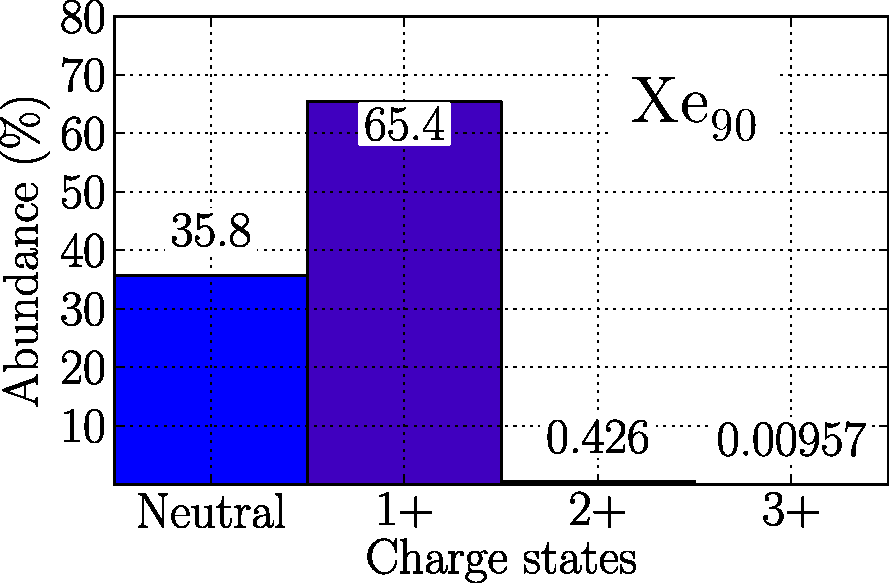
\includegraphics[width=\textwidth]{figures/figure_results_part2_CS_Xe100nmPart2BodstedIntensityScan_N00090_linear_ACI_OFF}}}
            {\uncover<3->{Without ACI:\newline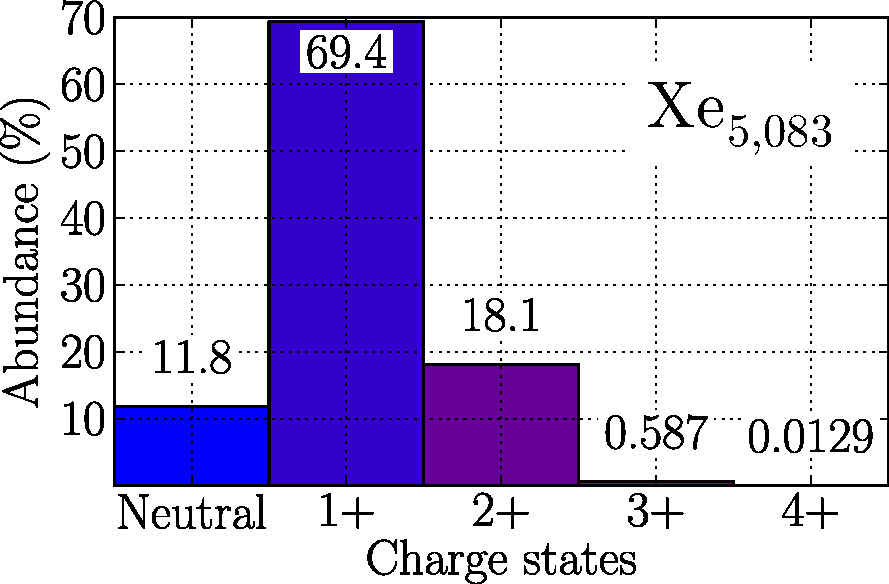
\includegraphics[width=\textwidth]{figures/figure_results_part2_CS_Xe100nmPart2BodstedIntensityScan_N05083_linear_ACI_OFF}}}
        \end{center}
        \column{0.4\textwidth}
        \begin{center}
            {\uncover<2->{With ACI:\newline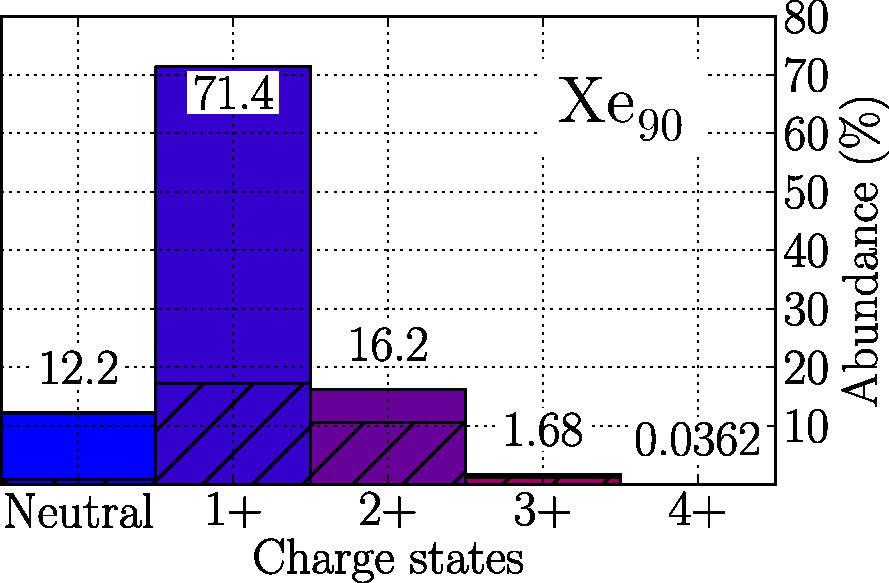
\includegraphics[width=\textwidth]{figures/figure_results_part2_CS_Xe100nmPart2BodstedIntensityScan_N00090_linear_ACI_ON}}}
            {\uncover<4->{With ACI:\newline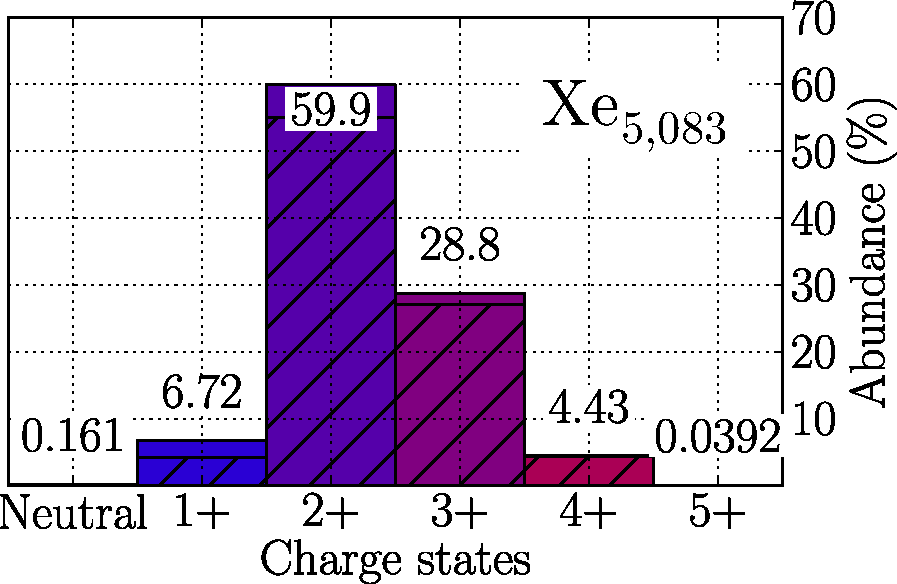
\includegraphics[width=\textwidth]{figures/figure_results_part2_CS_Xe100nmPart2BodstedIntensityScan_N05083_linear_ACI_ON}}}
        \end{center}
    \end{columns}
    \begin{center}
    \only<5>{
        % Place image @ page relative
        %                   (x, y)
        \begin{textblock}{0}(0.33,0.42)
        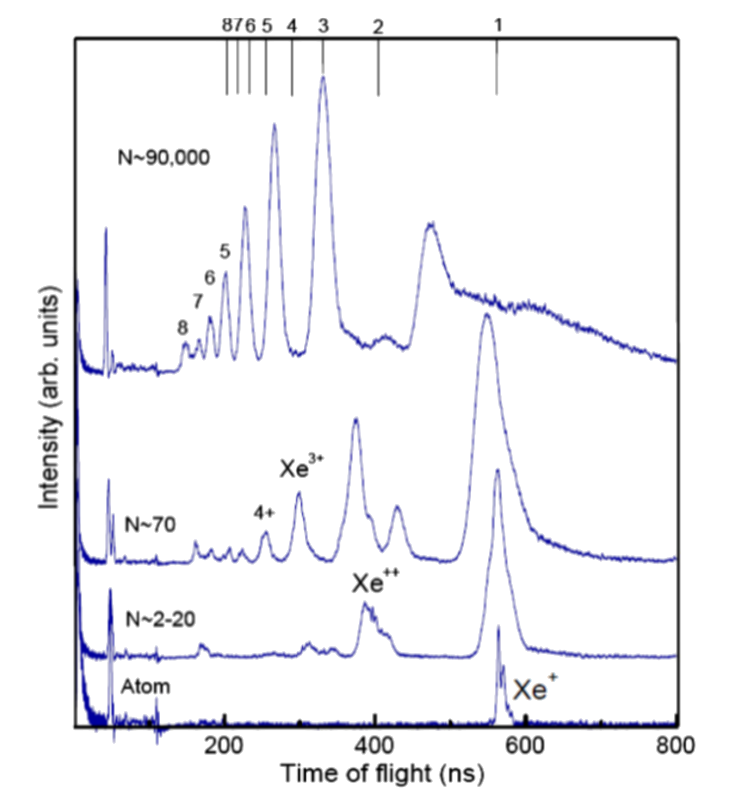
\includegraphics[width=0.3\paperwidth]{figures/Bostedt2010_fig2_opaque}
        \end{textblock}
    }
    \end{center}
\end{frame}







% ###############################################################
\subsection{Xenon @ XUV \& Recombination}
% ---------------------------------------------------------------
\subsubsection{Recombination}
% ***************************************************************
\begin{frame}{}\framenumber\setbeamercovered{invisible}
   \begin{columns}
       \column{0.6\textwidth}
       \begin{itemize}
           \item Thomas \textit{et al.} J. Phys. B (42) 13 134018 (2009)
           \begin{itemize}
            \item Coulomb explosion of outer-shell
            \item Core expansion $\rightarrow$ Recombination important
           \end{itemize}
           \item<2-> @ 13.7 nm (90.5 eV) \\ $\rightarrow$ $\sigma_\gamma$(4d) $\sim$ 10$\sigma_\gamma$(5p)
       \end{itemize}

       \column{0.5\textwidth}

        \begin{center}
            \begin{overlayarea}{\textwidth}{\textheight}
            \vspace{30pt}
            \only<1>{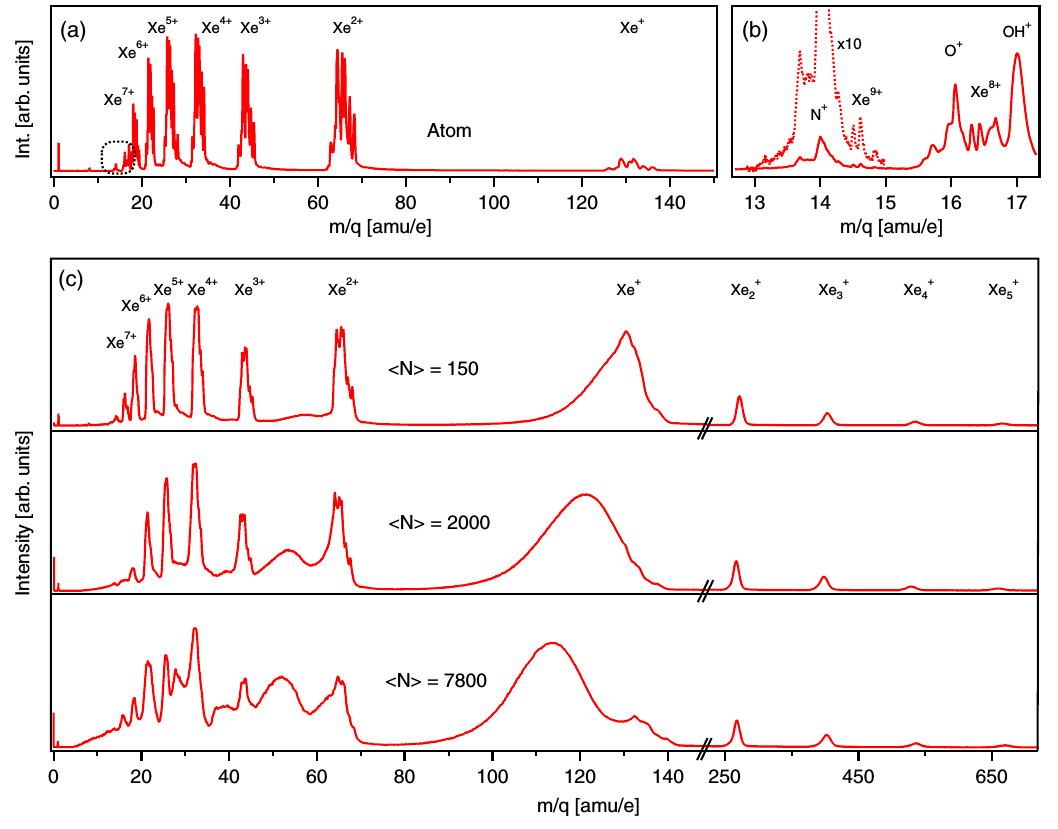
\includegraphics[width=\textwidth]{figures/Thomas2009_fig1}}
            \only<2>{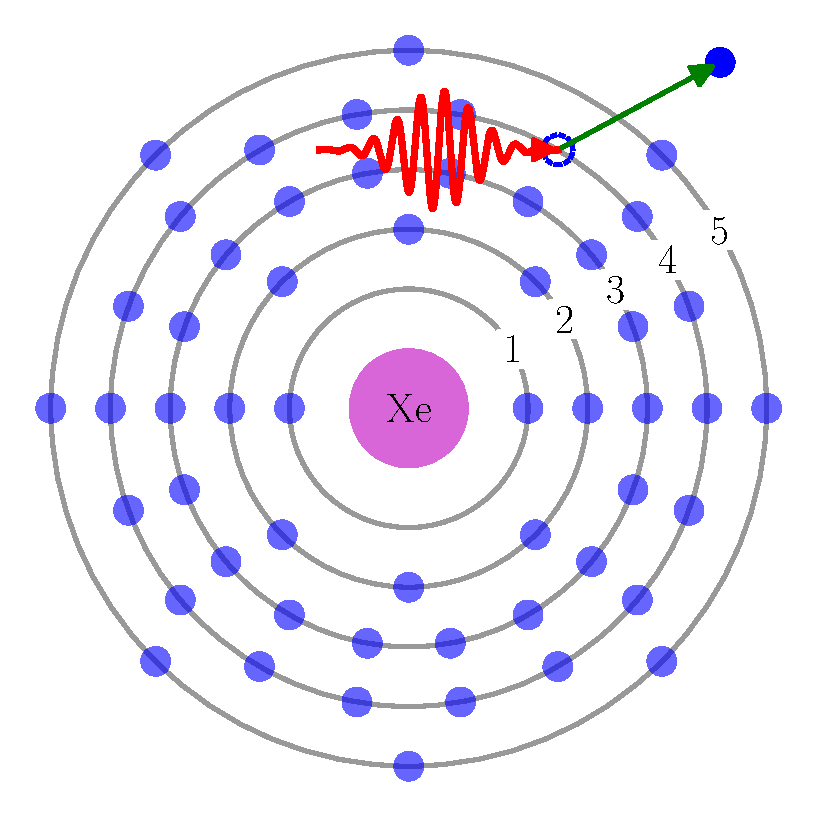
\includegraphics[width=0.7\textwidth]{../figures/auger_step_1}}
            \only<3>{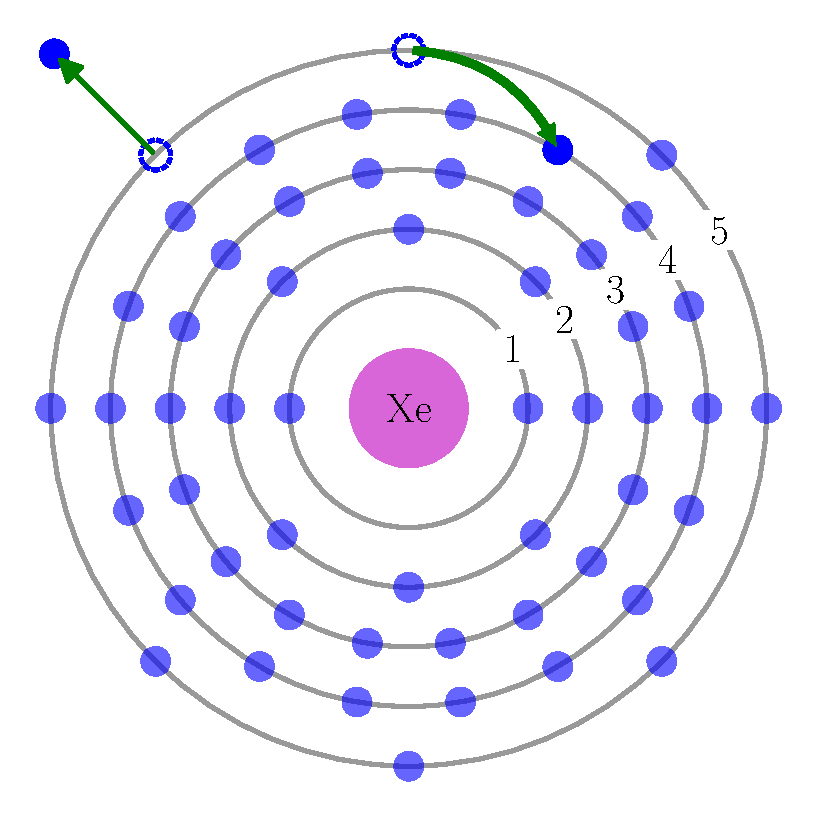
\includegraphics[width=0.7\textwidth]{../figures/auger_step_2}}
            \uncover<2->{\\ \centering Auger decay}
            \end{overlayarea}
        \end{center}

   \end{columns}
\end{frame}
% ***************************************************************
\begin{frame}{}\framenumber\setbeamercovered{invisible}
   \begin{columns}
       \column{0.6\textwidth}
       \begin{itemize}
           \item Xe$_{147}$, 10~fs, 13.7~nm (90.5~eV), 5.8$\times$10$^{14}$~W/cm$^2$
           \item<3-> Xe$^{7+}$ \& up: $\ge$5$\times$10$^{13}$~W/cm$^2$
           \item<3-> Xe$^{7+}$: $\sim$30~\% from 3$\times$10$^{14}$~W/cm$^2$
           \item<3-> Xe$^{10+}$ \& up: exclusively from 3$\times$10$^{14}$~W/cm$^2$
       \end{itemize}

       \column{0.5\textwidth}

        \begin{center}
            \uncover<2->{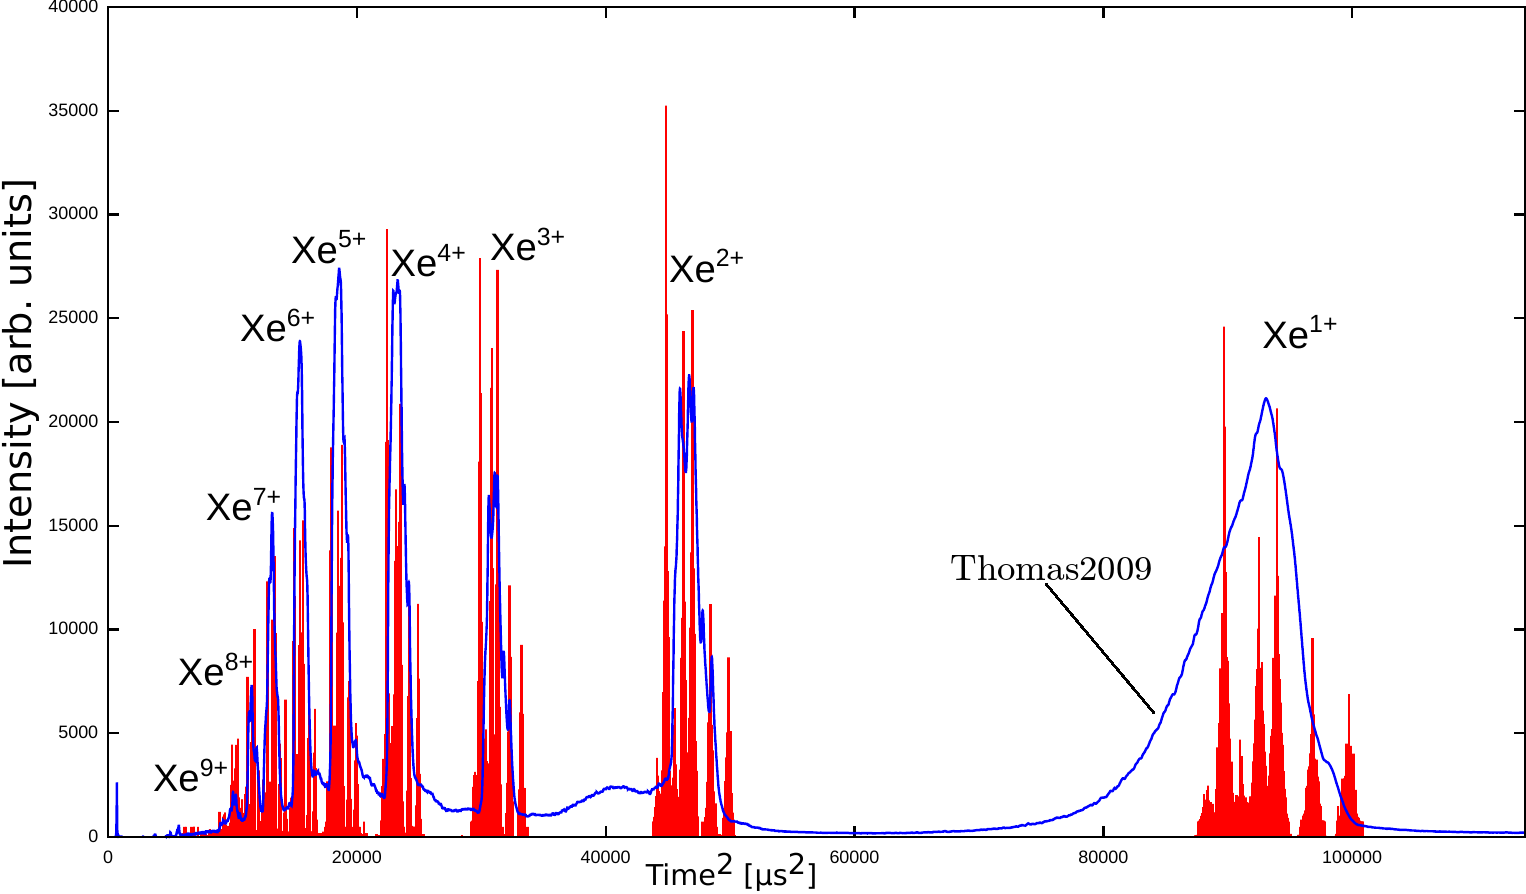
\includegraphics[width=\textwidth]{figures/Ackad2013_fig3}}
            \uncover<3->{\includegraphics[width=\textwidth]{figures/Ackad2013_fig4b}}
        \end{center}

   \end{columns}
\end{frame}
% ***************************************************************
\begin{frame}{}\framenumber\setbeamercovered{invisible}
Recombination effects (entire profile)
   \begin{columns}
       \column{0.8\textwidth}
        \includegraphics[width=\textwidth]{figures/Ackad2013_fig9}

        \uncover<2->{\begin{tiny}E. Ackad, N, Bigaouette, S. Mack, K. Popov and L. Ramunno. New Journal of Physics 15(5), 2013, 053047\end{tiny}}


        \column{0.37\textwidth}
        \begin{itemize}
           \item 3$^{\textrm{rd}}$ shell: Highest CS
           \item Center: High CS but recombine $\rightarrow$ Low CS
           \item 3$^{\textrm{rd}}$ shell: Low CS mostly from low Int. regions
           \item Outer shells: $\searrow$~density $\Rightarrow$ $\searrow$~recomb.
       \end{itemize}

   \end{columns}
\end{frame}


% % ###############################################################
% \section{Quantum Solver}
% ---------------------------------------------------------------
\subsection{QFDTD}
% ***************************************************************
\begin{frame}{}\framenumber
   \begin{columns}[t]
       \column{0.6\textwidth}
       \begin{itemize}
           %\item<+-> Atomic ionization $\sigma$?
           \item<1-> Cluster environment?
           \item<1-> Quantum mechanical effects?
           \item<2-> Finite-Difference Time-Domain (FDTD)
            \begin{itemize}
            \item<2-> Explicit solver (from E\&M) $\rightarrow$ Simple \& Easily //
            \item<2-> Geometry independence
            \end{itemize}
       \end{itemize}

       \column{0.5\textwidth}
       \begin{itemize}
           \item<1-> Neighbours' influence?
           \item<1-> Validation of our models?
           \item<3-> Maxwell's equations $\rightarrow$ \schrodinger equation
           \item<3-> Solve for the 1-e$^{-}$ wavefunction $\ket{ \psi\pa{\vecr,t} }$
       \end{itemize}
   \end{columns}

\uncover<3->{
\begin{center}
    $\im \delt{} \ket{ \psi\pa{\vecr,t} } = \pa{ - \frac{1}{2} \laplacien{} + V\pa{\vecr,t} } \ket{ \psi\pa{\vecr,t} }$
\end{center}
}

\uncover<4->{
Discretization 1 $\rightarrow$ Real time algorithm \\
Discretization 2 $\rightarrow$ Imaginary time algorithm
}
\end{frame}


% ---------------------------------------------------------------
\subsubsection{Real time vs Imaginary time}
% ***************************************************************
\begin{frame}{}\framenumber\setbeamercovered{invisible}
   \begin{columns}[t]

   \column{0.5\textwidth}
   Real time:
       \begin{itemize}
           \item $\psi_R\pa{\vecr,t}$ \& $\psi_I\pa{\vecr,t}$
           \item FT $\rightarrow$ eigenvalues
           \item Running FT $\rightarrow$ states
       \end{itemize}
    \vspace{20pt}
    \includegraphics[width=\textwidth]{figures/radial_5p_node}%\\
    %Whole domain: all states!


   \column{0.6\textwidth}
   \uncover<2->{
   Imaginary time:
       \begin{itemize}
           \item Wick rot. $\pi$/2 (complex plane)
           \item $\psi\pa{\vecr,\tau}=\sum_{n}\e{-E_n \tau}c_n\phi_n\pa{\vecr}$
           \item Eigenstates \& Eigenvalues
           %\item New method to extract excited states
       \end{itemize}

    \includegraphics[width=\textwidth]{figures/exponential_growths}
    }
   \end{columns}
\end{frame}

% ---------------------------------------------------------------
\subsubsection{Mapping}
% ***************************************************************
\begin{frame}{}\framenumber\setbeamercovered{invisible}

    \begin{columns}[t]
    \column{0.5\textwidth}
        Important contributions:
        \begin{enumerate}
            \item<+-> Actual implementation! $\sim$16k LoC
            \item<+-> RT: Whole domain for spectrum (linearity~of~FT)
            \item<+-> IT: New method for states extraction
            \item<+-> Both: Mapping of memory index $\leftrightarrow$ space from arbitrary source function
        \end{enumerate}

    \column{0.5\textwidth}
    \begin{center}
        {\uncover<2->{\includegraphics[width=0.9\textwidth]{figures/radial_5p_node}}}\\
        {\uncover<3->{\includegraphics[width=0.8\textwidth]{figures/exponential_growths}}}\\
        {\uncover<4->{\includegraphics[width=\textwidth]{figures/mapping}}}\\
    \end{center}

    \end{columns}

\end{frame}

% ---------------------------------------------------------------
\subsubsection{Results}
% ***************************************************************
\begin{frame}{Real time}\framenumber\setbeamercovered{invisible}
\includegraphics[width=0.75\textwidth]{figures/h_spectrum}\\
\begin{flushright}
\uncover<2->{\includegraphics[width=0.75\textwidth]{figures/h2p_spectrum}}
\end{flushright}
\end{frame}

% ***************************************************************
\begin{frame}{Imaginary time}\framenumber\setbeamercovered{invisible}
   \begin{columns}[t]
    \column{0.5\textwidth}
        \begin{center}
        H \\
        \includegraphics[width=0.95\textwidth]{figures/h_eigenstates}

        \begin{textblock}{0.2}(0.291,0.575)
        % ffmpeg -i h_3d.gif -qscale:v 1 -r 30 h_3d.swf
        \includemedia[label=H,activate=pagevisible,deactivate=onclick,width=\textwidth]
                     {\includegraphics{figures/h_3d.png}}{figures/h_3d.swf}
        \end{textblock}
        \end{center}

    \column{0.5\textwidth}
    \uncover<2->{
        \begin{center}
        H$_{2}^{+}$ \\
        \includegraphics[width=0.95\textwidth]{figures/h2p_eigenstates}\\
        {
        \begin{tiny}
        \begin{tabular}[c]{|c|c|c|c|}\hline
            States                      & $<E>$     & $<E_{\textrm{NL}}>$ & Error \\\hline\hline
            1 s $\sigma_{\textrm{g}}$   & -1.1026   & -1.1054  & 0.25~\% \\ \hline
            2 p $\sigma_{\textrm{u}}$   & -0.66753  & -0.67034 & 0.42~\% \\ \hline
            2 p $\pi_{\textrm{u}}$      & -0.42877  & -0.43055 & 0.41~\% \\ \hline
            2 s $\sigma_{\textrm{g}}$   & -0.36086  & -0.36242 & 0.43~\% \\ \hline
            3 p $\sigma_{\textrm{u}}$   & -0.25541  & -0.25887 & 1.3~\% \\ \hline
        \end{tabular}
        \end{tiny}
        }
        \end{center}
        \scalebox{.4}{
        Madsen \textit{et al.} Atomic Data and Nuclear Data Tables 2 (1970): 171–204
        }
    }
    \end{columns}

\uncover<2->{
\begin{tiny}Bigaouette \textit{et al.} Computer Physics Communications, 183(1), 2012, 38--45\end{tiny}
}
\end{frame}




% ###############################################################
\section{Conclusion}
% ***************************************************************
\begin{frame}{}\framenumber

\begin{columns}[t]

\column{0.5\textwidth}
    \begin{itemize}
    \item<+-> Wrote from scratch 2 simulation packages + libraries
    \item<+-> MD:
        \begin{itemize}
        \item<.-> Rare gas type
        \item<.-> Cluster sizes
        \item<.-> New model: ACI
        \end{itemize}
    \item<+-> QFDTD:
        \begin{itemize}
        \item<.-> 1 e$^{-}$ systems
        \item<.-> Novel mapping technique
        \end{itemize}
    \end{itemize}

\column{0.5\textwidth}
    \begin{itemize}
    \item<+-> Both: GPU accelerated
    \item<.-> Experimental results are reproduced
    \item<.-> Many publications
    \item<.-> MD:
        \begin{itemize}
        \item<.-> ACI $\lambda$ independent: Other regimes?
        \item<.-> Bigger clusters? Tree?
        \end{itemize}
    \item<.-> QFDTD:
        \begin{itemize}
        \item<.-> States inside bigger clusters
        \item<.-> Transition rates
        \item<.-> Cross-sections
        \end{itemize}
    \end{itemize}

\end{columns}
\end{frame}


% ###############################################################
\section*{Acknowledgements}
% ***************************************************************
\begin{frame}{}\framenumber

\includegraphics[width=\textwidth]{figures/phd052107s}

\begin{columns}[t]

\column{0.5\textwidth}
\begin{itemize}
\item University of Ottawa
\item Prof. Lora Ramunno
\item Thesis committee
\end{itemize}

\column{0.5\textwidth}
\begin{itemize}
\item Scholarships
\item Family and friends
\item Christine
\end{itemize}

\end{columns}
\end{frame}






% ###############################################################
% ###############################################################
% ###############################################################
\appendix


% ###############################################################
\section{QFDTD}
% ---------------------------------------------------------------
\subsection{Discretization}
% ***************************************************************
\begin{frame}{}\framenumber
\begin{center}
$\im \delt{} \ket{ \psi\pa{\vecr,t} } = \pa{ - \frac{1}{2} \laplacien{} + V\pa{\vecr,t} } \ket{ \psi\pa{\vecr,t} }$

\begin{align}
\ket{ \psi\pa{\vecr,t} } & =        \ket{ \psi_R\pa{\vecr,t} }
                            + \im \ket{ \psi_I\pa{\vecr,t} } .
\end{align}

\end{center}
\end{frame}

% ---------------------------------------------------------------
\subsection{Imaginary time: New method for eigenstates calculation}
% ***************************************************************
\begin{frame}{}\framenumber
\begin{center}
\begin{align}
\ket{ \psi\pa{\tau_n}' } & = \ket{ \psi\pa{\tau_n} }
                        - \ket{\phi_0} \crossp{\phi_0}{\psi\pa{\tau_n}} \\
\ket{ \psi\pa{\tau_n}'' } & = \ket{ \psi\pa{\tau_n}' }
                        - \ket{\phi_0} \crossp{\phi_0}{\psi\pa{\tau_n}'}
                        - \ket{\phi_1} \crossp{\phi_1}{\psi\pa{\tau_n}'}
\end{align}
\end{center}
\end{frame}



\end{document}
